% !TeX encoding = UTF-8
% !TeX program = pdflatex
% !TeX spellcheck = en_US

\documentclass[LaM,binding=0.6cm]{./packages/sapthesis/sapthesis}

\usepackage{microtype}
\usepackage{amssymb}
\usepackage{amsmath}
% Norm Command
\newcommand{\norm}[1]{\left\lVert#1\right\rVert}

\usepackage{hyperref}
\hypersetup{pdftitle={Robustness of Deep Neural Networks Using Trainable Activation Functions},pdfauthor={Federico Peconi}}


% Remove in a normal thesis
\usepackage{lipsum}
\usepackage{curve2e}
\usepackage{algpseudocode}
\usepackage{dblfloatfix}
\usepackage[backend=biber]{biblatex}
\addbibresource{adversarial.bib}
\definecolor{gray}{gray}{0.4}
\newcommand{\bs}{\textbackslash}

% Commands for the titlepage
\title{Robustness Of Deep Neural Networks \\Using Trainable Activation Functions}
\author{Federico Peconi}
\IDnumber{1823570}
\course{Computer Science}
\courseorganizer{Computer Science - Informatica LM-18}
\AcademicYear{2019/2020}
\copyyear{2020}
\advisor{Prof. Simone Scardapane}
%\advisor{Dr. Nome Cognome}
%\coadvisor{Dr. Nome Cognome}s
\authoremail{peconi.1823570@studenti.uniroma1.it}

\examdate{Something October 2020}
\examiner{Prof. Nome Cognome}
\examiner{Prof. Nome Cognome}
\examiner{Dr. Nome Cognome}
\versiondate{\today}



\begin{document}

\frontmatter

\maketitle
\dedication{Dedicated to\\ Donald Knuth}

\begin{abstract}
This document is an example which shows the main features of
the \LaTeXe\ class \texttt{sapthesis.cls} developed by 
with the help of GuIT (Gruppo Utilizzatori Italiani di \TeX).
\end{abstract}

\begin{acknowledgments}
Ho deciso di scrivere i ringraziamenti in italiano
per dimostrare la mia gratitudine verso i membri
del GuIT, il Gruppo Utilizzatori Italiani di \TeX, e, in particolare,
verso il prof. Enrico Gregorio.
\end{acknowledgments}

\tableofcontents

% Do not use the starred version of the chapter command!
%\chapter{Capitolo non numerato}

\mainmatter

\chapter{Introduction}

    \section{Intriguing Properties of Neural Networks}

        The vast majority of cutting-edge \textit{neural network} based classifiers is currently vulnerable to imperceptible non-random perturbations of the input.
        As first shown by C. Szegedy \textit{et al.} in \cite{szegedy2013-intriguing}, and then subsequently in many other publications \cite{journals/corr/NguyenYC14}, \cite{journals/corr/BiggioCNRMFGR14},
        it is sufficient for an \textit{adversary} to add a small amount of targeted noise on a sample in order to induce the model to predict, with high confidence,
        a wrong class. Despite the fact that such \textit{attacks} are relevant in many different domains, ranging from natural language processing \cite{nlp_adv} to automatic speech recognition \cite{speechrec_adv}, 
        it is typical to introduce the problem with concrete examples dealing with images.
        Indeed, within the framework of image classification, perturbations have a nice interpretation in terms of norms and the problem itself can be appreciated visually.
        For instance, assume to have an image $x$ of a \textit{dog} and a performant classifier which correctly recognizes the subject. Then, by means of a few lines of code\footnote{Using modern Deep Learning libraries.},
        it is possible to devise a pixel-wise perturbation such that: the resulting perturbed image looks perfectly the same to the human eye and yet, it gets misclassified --by the same model with strong conviction--
        as it is depicting a \textit{cat} Fig. \ref{fig:aecatdog}.  
        \begin{figure}[!h]
            \centering
            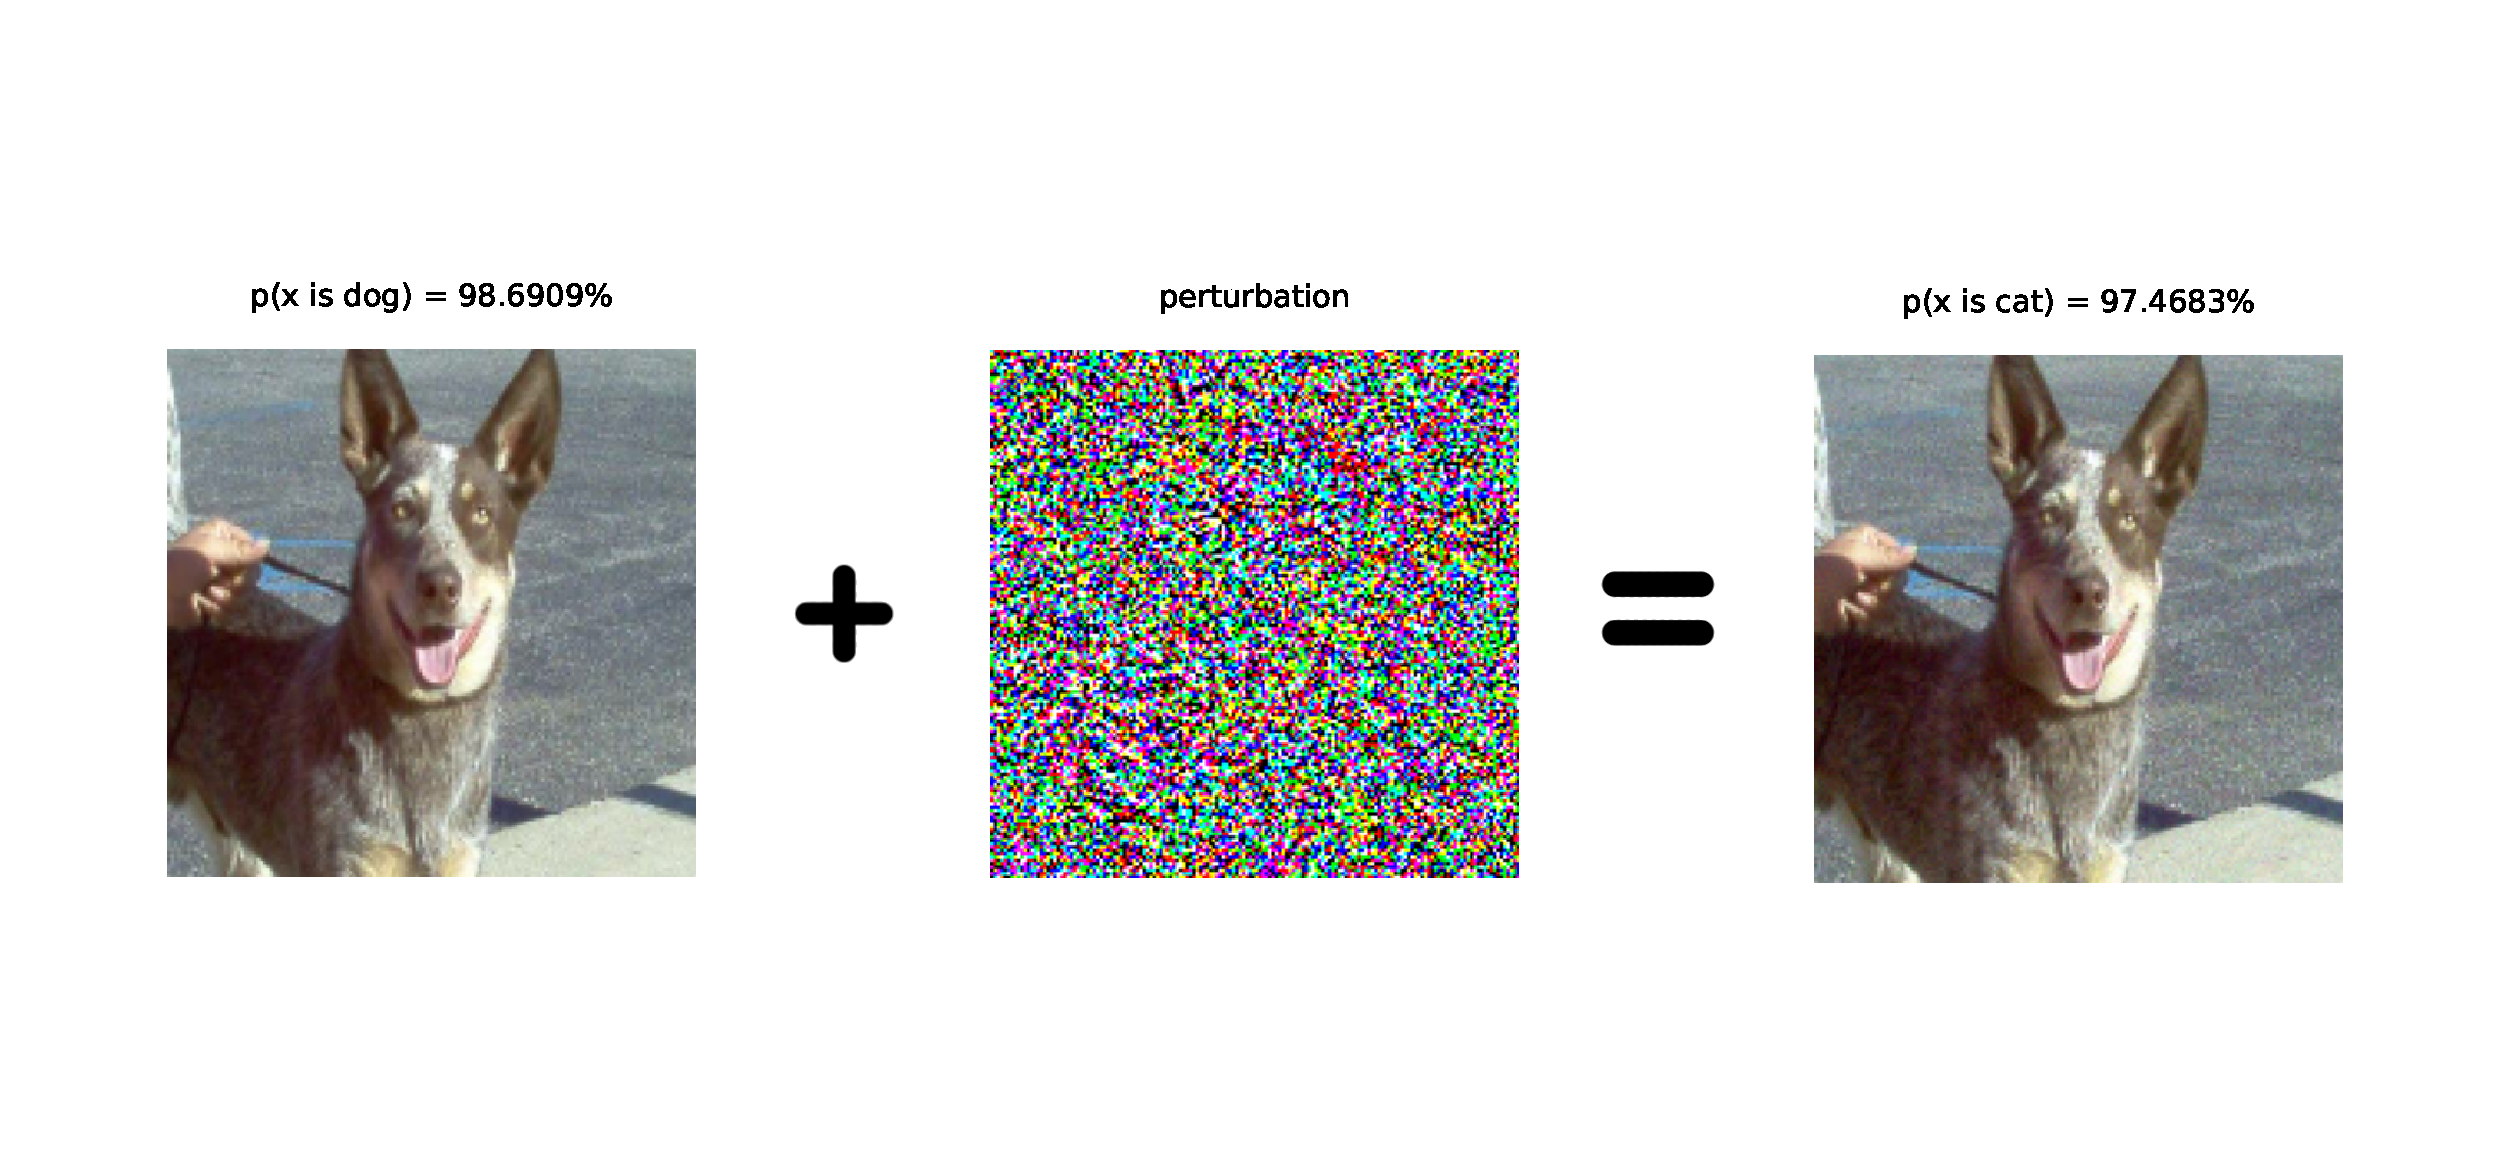
\includegraphics[width=0.95\textwidth]{prt.png}
            \caption{By means of a noisy perturbation of the image, an image classifier model can be fooled into believing with high confidence that what was correctly labeled as a dog is now a cat.}
            \label{fig:aecatdog}
        \end{figure}
        More alarming is the fact that such misclassifications can be targeted, just as easily, by the adversary towards any desired class. Any crafted input designed to 
        cause an incorrect output is called an \textit{adversarial example}.

        Adversarial examples pose a vital threat for the deployability of autonomous systems in safety-critical applications. In \cite{iCub} real-world adversarial examples for 
        a humanoid robot are proposed whereas \cite{darts} and \cite{autonomous_adv} illustrate the feasibility of fooling autonomous-driving car systems.
        Moreover, as the performances of intelligent systems increase \cite{residual_nets} \cite{inception}, and their availability becomes ever more within the reach of --fundamentally-- anyone who can connect to the internet, these algorithms 
        are already finding their way into other security-critical scenarios such as aerial vehicles facial authentication \cite{aerialveichles}, social engineering detection, network anomaly detection \cite{socialeng_adv} \cite{anomalydet_adv} and so on. 
        Thus, making them all prone to suffer from some kind of adversarial attack, if no defense technique is explicitly implemented.
        
        Along with the obvious security concerns that we have just discussed, there is another fundamental reason to develop methods capable of preventing adversarial examples, which is, the opportunity of 
        building more human-aligned models. Any claim about state-of-the-art classifiers that have surpassed "human performances" is indeed far from being true, if we look at the task through the lens of adversarial examples.
        In particular, any person would have no trouble in correctly classifying an adversarially perturbed image on which state-of-the-art models are consistently fooled. That is likely because humans tend to learn features that are 
        extremely resilient towards sampling distribution changes, whereas neural networks are eventually prone to learn brittle, sampling-specific features \cite{features_notbugs}.
        Moreover, recent works have showed how the \textit{interpretability} of a model, which is usually very difficult to assess in performant deep neural networks, is instead significantly increased 
        when we evaluate \textit{adversarially robust} networks \cite{robustness_accuracy} \cite{interpret_adv}. Therefore, broadly speaking, adversarial examples 
        seem to be only a symptom of the discrepancy between the way humans and intelligent systems currently learn.

        Nowadays, despite the relevance for the field, no truly robust model for real-world applications has been developed yet. For CIFAR10, a relatively small toy dataset used in image classification, 
        the current state-of-the-art model achieves 43.96\% of accuracy against the most effective attack \cite{cifar10challange}.
        Furthermore, things get even more complicated when we try to scale up to larger, more realistic models, since it generally becomes extremely expensive to train robust models in these settings \cite{free_adv_train}.
        Specifically, it is commonly believed that, to improve robustness, one needs to either largely extend the size of the dataset or increase the network capacity \cite{scaleintriguing}.
        Due to the lack of a global understanding of the nature of adversarial examples, the critical security alarms that arise with them and the complexity of developing effective defenses,
        the area of adversarial robustness is constantly attracting more and more research interest \cite{towards_eval_robustness}.


    \section{Activation Functions and Robustness}

        In this thesis, we focus on analyzing the effects of structural changes in deep neural networks, in terms of adversarial robustness.
        In particular, we try to assess how \textit{adversarial training} \cite{madry_adv_training}, i.e., the act of training using adversarial examples,
        may benefit from theoretically principled changes in the model's architecture.
        As previously anticipated, one known method to boost the resiliency --during such training-- consists in naively adding more capacity to the model, by simply 
        introducing more parameters.  
        However, such a technique requires to build a significantly bigger network which is ultimately different from the original one. On the contrary, we are concerned with 
        minor modifications, leaving the overall structure unchanged.

        Recently, a link between activation functions and robustness has been proposed. In \cite{smooth_adversarial_training}, authors showed that it is possible to strengthen
        adversarial training by means of activation functions that are \textit{smooth} or, in other words, functions whose first derivative is continuous everywhere\footnote{Formally we say these functions are $\mathcal{C}^1$ continuous.}. 
        Indeed, their experiments consistently reported greater performances when, instead of the 
        typical rectified linear unit (ReLU) \cite{relu}, the model's non-linearities were substituted by a smooth counterpart, such as: ELU, GELU or Swish functions \cite{elu} \cite{gelu} \cite{swish}.
        It is worth to note that such improvement comes for "free", in the sense that no data augmentation or network growth were carried out, in contradiction with 
        the common wisdom \cite{freelunch}.
        
        Building up from this result, we propose the evaluation, within the same framework, of a novel class of activation functions called \textit{kernel-based activation functions} (KAFs).
        KAFs were first introduced in \cite{kafnets} as a promising class of trainable activation functions, aiming to overcome the limitations of other alternatives present in the literature. 
        In particular, trainable activation functions are non-linearities whose shape can be trained together with the other weights of the network, by means of 
        trainable parameters present in the formulation. By leveraging cheap kernel expansions, the locality effects of their parameters and other desirable 
        properties, KAFs allows for fast convergence, universal shape approximations and generalization of the network \cite{kafnets_generalization}.
        Compared to the fixed and trainable counterparts, KAFs result in better empirical performances on a variety of tasks \cite{kafnets}. Ultimately,
        KAFs can be made smooth with the employment of smooth kernels, such as the 1-dimensional Gaussian kernel.

        Through a combination of both flexibility --resulting from their trainable nature-- and smoothness, we argue that the adversarial training of
        deep neural networks will benefit from the presence of KAFs inside the model's architecture.
        
    \section{Structure of the Thesis}

    From a high-level, this thesis is divided into two parts. The first part, which ranges from Chapter \ref{chap:2} to Chapter \ref{chap:4}, introduces the reader 
    to the basic concepts needed in order to understand the second part, where main ideas are developed and evaluated. The latter starts from Chapter \ref{chap:5} and ends with Chapter \ref{chap:8}.
    Specifically, Chapter 2 discusses the fundamentals of Deep Learning, Chapter \ref{chap:3} the formal theory of adversarial examples and Chapter 4 is a brief review of
    fixed and parametric activation functions, focusing in particular on KAFs. The reader familiar with the relevant literature and notation on adversarial 
    examples (Szegedy et al., 2014; Carlini  Wagner, 2017b; Madry et al. Athalye et al., 2018a, etc.), can safely skip to Chapter 4.
    Following, Chapter 5 gives a detailed description of the related works which corroborate our hypothesis, Chapter \ref{chap:6} introduces theoretical 
    and empirical insights on why we conjecture the potentials of KAFs, and finally in Chapter \ref{chap:7}, experiments, using different architectures, 
    are presented and commented. Chapter 8 concludes the work by drawing a final comment on the results obtained, contributions 
    as well as the shortcomings faced and relevant ideas for future works.

\part{Fundamentals}


\chapter{Neural Networks}
        \label{chap:2}
        Broadly speaking, the field of Machine Learning is the summa of any algorithmic methodology whose aim is to automatically find meaningful patterns inside data without
        being explicitly programmed on how to do it. Well known examples are: Decision Trees \cite{decision_tree}, Support Vector Machines \cite{svm}, Clustering \cite{clusters},
        Neural Networks \cite{perceptron} and, more recently, 
        Deep Neural Networks \cite{deepnn}. During the last two decades Deep Neural Networks have gained a lot of attention for their outstanding performances in different tasks like
        image classification \cite{imagenet}, speech and audio processing \cite{dlaudioprocessing}.

        \section{Definition}
            
            Neural Networks (NNs) are often used in the context of Supervised Learning where the objective is to model a parametric function 
            $ f_{\theta} \colon \mathcal{X} \to \mathcal{Y}$ given $n$ input-output pairs $S = \{(x_i, y_i)_{i=1}^n\} $ with $x_i \in \mathcal{X}$ and $ y_i \in \mathcal{Y}$
            such that
            \begin{equation}
                f_{\theta} \sim f,
            \end{equation}
            where $f$ is assumed to be the real input-output distribution that we want to learn. In plain words, this means that we want to find the best set of parameters $\theta^{*}$ for the model
            such that, for any unseen input $x_{new}$ we have that $f_{\theta^*}\left(x_{new}\right)$ is as close as possible to $f\left(x_{new}\right)$

            For the sake of explanation, assume the input, which in practice can be very complex and unstructured e.g. made of: graphs, text, sounds, etc, to be embedded in an input space  $\mathcal{X} = \mathbb{R}{^d}$.
            The simplest form of a neural network is then given by
            \begin{equation}
                \label{layer}
                f_{W, b}\left(x\right) = \sigma(Wx + b),
            \end{equation}
            where the parameters of the network are the elements of a $u \times d$ matrix $ W $ and a $u$-dimensional vector called bias. The last element $ \sigma $ applied at the end is a
            function which consists of a non-linear function acting element-wise and is the key component to introduce non linearity in NNs allowing them to model 
            highly non-linear functions. We call it \textit{activation function}. \ref{layer} can then be rewritten:
            \begin{equation}
                f_{W, b}\left(x\right) = \left[\sigma(W_1^{\intercal} x + b_1), \sigma(W_2^{\intercal} x + b_2), \ldots, \sigma(W_u^{\intercal} x + b_u)\right],
            \end{equation}
            where $W_i$ and $b_i$ are respectively the i-th row of $W$ and the i-th element of the bias.
            
            Historically, the whole picture was somehow biologically inspired and had an intuitive explanation. Indeed, if we think at $ W $ as weights i.e. $ w_{ij} $ as the importance
            the model gives to the input $x_i$ for how much it contributes to the $ f_{W}\left(x\right)_j $-th component and define $ \sigma $ to be
            \begin{equation}
                \label{step}
                \sigma(W_j^{\intercal} x + b_j) = \begin{cases} 
                    1 & W_j^{\intercal}x \geq - b_j \\
                    0 & W_j^{\intercal}x < - b_j 
                \end{cases},
            \end{equation}
            then it is easy to see that here the bias is acting like a threshold which discrminates between \textit{activating} or not the $j$-th component depending on how much importance was given. 
            Due to this analogy with the behaviour of neurons in the brain we call each component \textit{neuron}, non-linearities activation functions and the whole model neural network.
            \begin{figure}[h]
                \centering
                \includegraphics[width=0.5\textwidth]{slide1}
                \caption{Graphic representation of a one layer NN also know as MLP.}
            \end{figure}
            \paragraph{}
            In general, the idea of a layer of neurons can be recursively extended by stacking more layers together, all of which are described by a matrix of weights, a bias and an activation function
            and letting the output of one becoming the input of the subsequent.
            The resulting model is the mathematical composition of the layers, thus if we let $ L $ be the number of layers, $ z_0 = x $ and $ z_l = \sigma_l\left(W_{l}z_{l-1} + b_l\right)$
            we write a $L$-layered $f_{\mathbf{W}, \mathbf{b}}$:
            \begin{equation}
                f_{\mathbf{W}, \mathbf{b}} = z_L = \sigma_{L}\left(W_{L}\sigma_{L-1}\left(\ldots\left(W_2\sigma_{1}\left(W_{1}z_{0} +b_1\right)+ b_2\right)\ldots\right)+ b_{L}\right).
            \end{equation}
            With $ \mathbf{W} = \{W_1, \ldots, W_{L}\} $ and $ \mathbf{b}= \{b_1, \ldots, b_{L}\} $. We will call the first layer \textit{input layer}, the middle layers \textit{hidden layers}
            and the last layer \textit{output layer}.
            \begin{figure}[h]
                \centering
                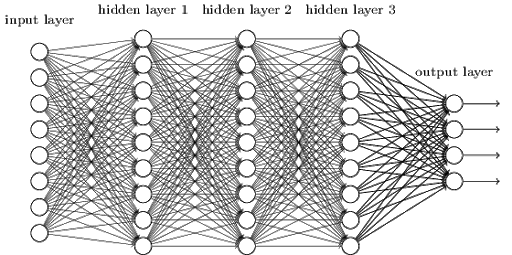
\includegraphics[scale=0.5]{fnn}
                \caption{A Feedforward Neural Network with 3 hidden layers. Source: Michael A. Nielsen, 'Neural Networks and Deep Learning, Determination Press', 2015}
                \label{fig:fnn}
            \end{figure}
            This general but still basic form of Neural Network is known as \textit{Feed Forward Neural Network} Fig. \ref{fig:fnn}. 
        \section{Training}

            There are still a couple of important pieces left to define to develop a properly working Neural Network. For instance, how are parameters computed? And in particular, with respect to what we compute them? 
            \subsection{Loss Function}
                Before we realized that our goal is to maximize the approximation of the ground-truth input-output relation that lies under the data, therefore there is a need to
                introduce some metric to quantify this approximization. Call \textit{loss function} $ L(f_{\theta}\left(x\right), y) \colon \mathcal{Y} \times \mathcal{Y} \to \mathbb{R_+}$ 
                such metric. Common choices are:
                \begin{itemize}
                    \item Least Square: $\norm{f_{\theta}\left(x\right) - y}^2$ for regression tasks 
                    \item Binary Cross-Entropy: $y \log (f_{\theta}(x))+(1-y) \log (1-f_{\theta}(x))$ for binary classification  
                    \item Categorical Loss Function: $-\sum_{c=1}^{C} y_{c} \log \left(f_{\theta}(x)_c\right)$ for multicategory classification with $C$ classes.
                \end{itemize}
                Intuitively, a good loss function will map bad approximations to high values and good approximations to smaller ones.
                Nevertheless, those are only point-wise estimates of the error, hence the best empirical solution learnable from the training set $ S $ would be 
                \begin{equation}
                    \label{erm}
                    \displaystyle{  \min_{\theta}  \frac{1}{n} \sum_{i=1}^{n} L\left(f_{\theta}\left(x_{i}\right), y_{i}\right) },
                \end{equation}
                which is called \textit{empirical risk minimization}.
            \subsection{Gradient Descent}
               So far we have described, given an input $ x $, how we can compute the output of a feedforward neural network by means of compositions of dot products 
               and non-linear transformations between matrices, starting from the first to the very last of the layers in what is called a \textit{forward pass}. As it turns out, to attempt to solve \ref{erm} we need to follow the exact
               opposite path. Indeed, every optimization algorithm used in practice makes use of the same subroutine called Backpropagation \cite{backprop} introduced in the 1970s, which allows to compute, starting from the output layer
               and going backwards, the partial derivative of the loss function with respect to each weight in the network. Moreover it does so efficiently requiring only one \textit{backward pass}.

               Let $i^l = W_l z_{l-1} + b_l$ be the weighted input to the $l$-th layer, then the key observation is that the only way $ W_l $ can affect the loss function is by affecting linearly
               the next layer which in turn affects its next layer and so on. In particular assume we add a little change $\Delta i_{j}^{l} $ to the $j$-th 
               element of $ i^l $ so that the neuron will output $ \sigma \left(i_{j}^{l} + \Delta i_{j}^{l}\right) $, this change will
               eventually propagates in the network causing the overall loss $LS$ to change by an amount $\frac{\partial LS}{\partial i_{j}^{l}} \Delta i_{j}^{l}$. For brevity,
               denote the gradient of the weighted input on the j-th neuron $ \delta^{l}_{j} = \frac{\partial LS}{\partial i^{l}_{j}} $, then the following holds:
               \begin{equation}
                 \delta^{L}_{j} = \frac{\partial LS}{\partial i^{L}_{j}} = \frac{\partial LS}{\partial z^{L}_{j}}\frac{\partial z^{L}_{j}}{\partial i^{L}_{j}} \\
                                =\frac{\partial LS}{\partial z^{L}_{j}} \sigma_{L}^{\prime}(i^{L}_{j}),
               \end{equation}
               and equally, taking into account the whole output layer
               \begin{equation}
                    \label{bp1}
                    \delta^{L}=\nabla_{z^L} LS \odot \sigma^{\prime}(i^{L}),
               \end{equation}
               where $ \odot $ is the element-wise product and $ \nabla_{x} $ the vector of the partial derivatives $ \partial LS / \partial x $. 
               That is, the gradient with respect to the weighted input to the last layer is given, using the chain rule, by the gradient with respect to the activation of the last layer times the derivative
               of the last activation function. Similarly, for any hidden layer $ l $ we note that:
               \begin{equation}
                \label{bp2}
                    \delta^{l}=\left((W^{l+1})^{T} \delta^{l+1}\right) \odot \sigma^{\prime}(i^{l}).
                \end{equation}
                When we apply the transpose weight matrix, $(W^{l+1})^{T}$, think intuitively of this as moving the previous layer's gradient backward, giving a measure of the gradient at the output of the $l$-th layer. 
                We then take the product $\sigma^{\prime}(i^{l})$ which again moves the gradient backward through the activation function in layer $l$, giving the gradient of the weighted input to layer $l$.

                By combining \ref{bp1} with \ref{bp2} we can compute the gradient $\delta^{l}$ for any layer in the network. We start by using \ref{bp1} to compute on the last layer, 
                then apply equation \ref{bp2} to compute $\delta^{L-1}$, then the same equation again to compute $\delta^{L-2}$, and so forth, 
                all the way back until the input layer. Since our intent is to retrieve the gradients for every weights of the network, we are left to 
                show how $ \delta^l $ relates to them, here we provide such relation without giving an explicit proof which instead can be found in many
                texts like \cite{nielsen2015neural}.
                \begin{equation}
                    \frac{\partial LS}{\partial b^{l}_{j}} = \delta^{l}_{j},
                \end{equation}
                \begin{equation}
                    \frac{\partial LS}{\partial w^{l}_{i,j}} = z^{l-1}_i \delta^{l}_{j}.
                \end{equation}
                Remark how we already know how to compute each element on the right sides of these equations, moreover, given that the activation function
                and its derivative is efficiently computable, we will be able to efficiently get the seeked gradients in just one pass.
                It is worth mention that Backpropagation is actually a special case of a more generic set of programming techniques that go under
                the name of \textit{Automatic Differentiation} \cite{adiff} to numerically evaluate the derivative of a function specified by a computer program.
                Such techniques are usually implemented in modern numerical libraries building variations of a data structure called \textit{computational graph}.
                Well known examples are \textit{Autograd} in \textit{Pytorch} \cite{pytorch} or \textit{GradientTape} in \textit{TensorFlow} \cite{tensorf}.

               What does it mean to be able to compute partial derivatives of the loss? It means being able to understand where and how 
               the loss decreases and thus we can exploit such information to find better and better weights solutions. 
               This is the idea behind the Gradient Descent algorithm \cite{sgd}. In particular, the gradient of a weight is nothing but the
               direction inside the weight-space where the loss function is increasing, therefore what we want to do is to follow the opposite
               direction. Formally, this translates in the following weight update rules:
               \begin{equation}
                    w^{t}_{l} \rightarrow w_{l}^{t+1}=w^{t}_{l}-\frac{\eta}{n} \sum_{j} \frac{\partial LS_{x_{j}}}{\partial w^{t}_{l}},
               \end{equation}
               \begin{equation}
                b^{t}_{l} \rightarrow b^{t+1}_{l}=b^{t}_{l}-\frac{\eta}{n} \sum_{j} \frac{\partial LS_{x_{j}}}{\partial b^{t}_{l}},
               \end{equation}
            where $w_{l}^{t}$ are the values of the weights for layer $l$-th during the $t$-th pass, $\eta$ is a small positive constant called \textit{learning rate}
            chosen by the user accordingly and the gradients are averaged among all samples in the training set. 
            \begin{figure}[h!]
                \centering
                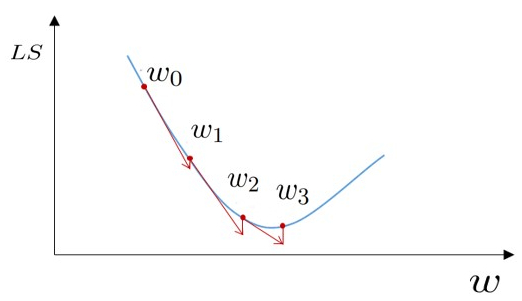
\includegraphics[scale=0.5]{gd}
                \caption{A 1-D representation of 4 gradient descent steps}
                \label{fig:gd}
            \end{figure}
            Most importantly, note how we take the negative of the gradients, meaning that we are following the direction in which the loss decreases Fig. \ref{fig:gd}. The distance
            between two consecutives weights $\Delta_{w^t}$ well be directly proportional to both the learning rate picked and the averaged gradient.

            In practice, however, very often we are dealing with thousands or millions of data points, becomes unfeasible to compute every pass over
            the entire training set, thus what is done is to split the data into so-called \textit{mini-batches} and then apply the
            update rules on each mini-batch until we scanned the whole data. The entire scan is called \textit{epoch} and the 
            resulting algorithm Stochastic Gradient Descent \cite{sgd}. Lastly, the size of a mini-batch is another hyperparameter 
            that should be tuned by the developer, keeping in mind that the bigger the size the more stable will be our training
            the smaller the size the faster the training.
            \begin{figure}[h]
                \centering
                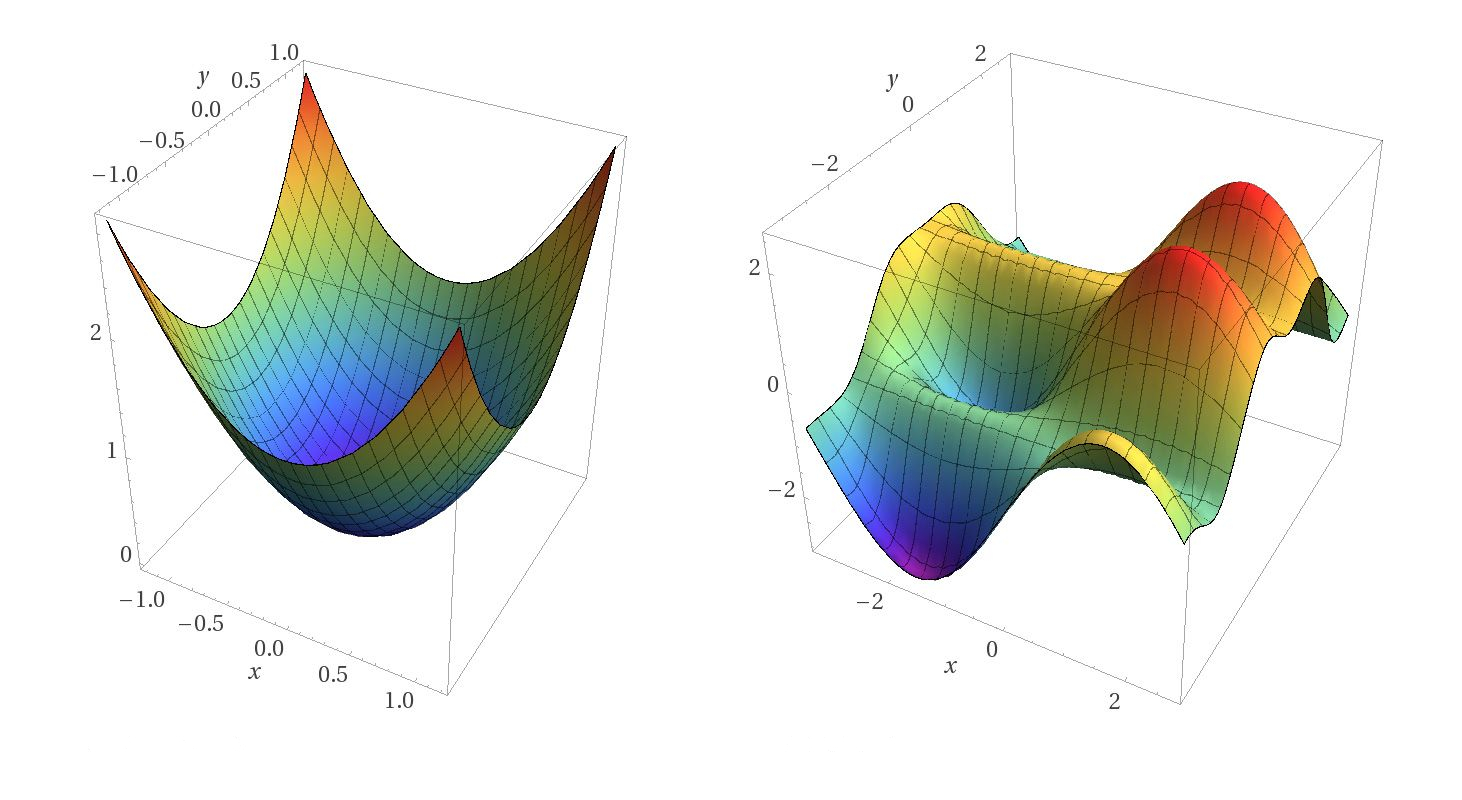
\includegraphics[scale=0.25]{conv_nonconv}
                \caption{Convex and Non-convex optimization landscapes}
                \label{fig:convnonconv}
            \end{figure}
            As stated earlier, neural networks can model extremely non-convex input-output functions therefore in principle there
            is no guarantee that Gradient Descent will find the optimal solution to \ref{erm} Fig. \ref{fig:convnonconv}.
            Indeed, the optimal solution would be the global minimum of our weighted loss function but there is no apparent
            way for the algorithm to distinguish between global, local minimum or saddle points Fig. \ref{fig:globlocsad}.
            However, it turns out that in practice Gradient Descent works fairly well once we correctly tune
            hyperparameters and run the algorithm from different initial values.
            Moreoever, lately authors have been proposed different methods to improve the convergence and the efficiency by 
            smart changes of the learning rate during the training process \cite{smith2017cyclical}. 
            \begin{figure}[h]
                \centering
                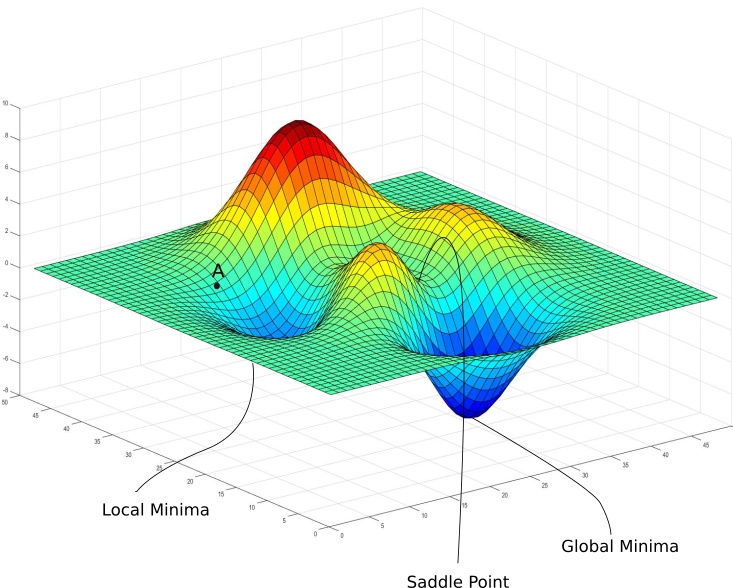
\includegraphics[scale=0.35]{globlocsad}
                \caption{Visualization of global, local and saddle points. How can A reach the global minimum?}
                \label{fig:globlocsad}
            \end{figure}

        \section{Activation Functions}
            
            We have seen how the learning process works optimizing the empirical risk by means of gradient computation.
            Therefore to be able to optimize anything, a neural network needs to have only differentiable components.
            However, before in \ref{step} we discussed the so-called \textit{step function}, an activation function that, 
            even if biologically inspired and easier to justify, is not differentiable at the origin and the derivative is 0 elsewhere.
            Thus if we think again about how Backpropagation works, we see that employing such an activation function would make the weight updates impossible
            since already $ \delta^{L} $ would be either undefined or 0.

            To deal with this issue, one of the first proposed activation functions was an approximation of the step function known as \textit{sigmoid}: 
            \begin{equation}
                \textnormal{sigmoid}(x) = \frac{1}{1 + e^{-x}},
            \end{equation}
            which is differentiable everywhere with continuous derivatives (property that we will refer as \textit{smoothness} through the chapters) and
            maps to $ [0, 1] $ values.
            \begin{figure}[h]
                \centering
                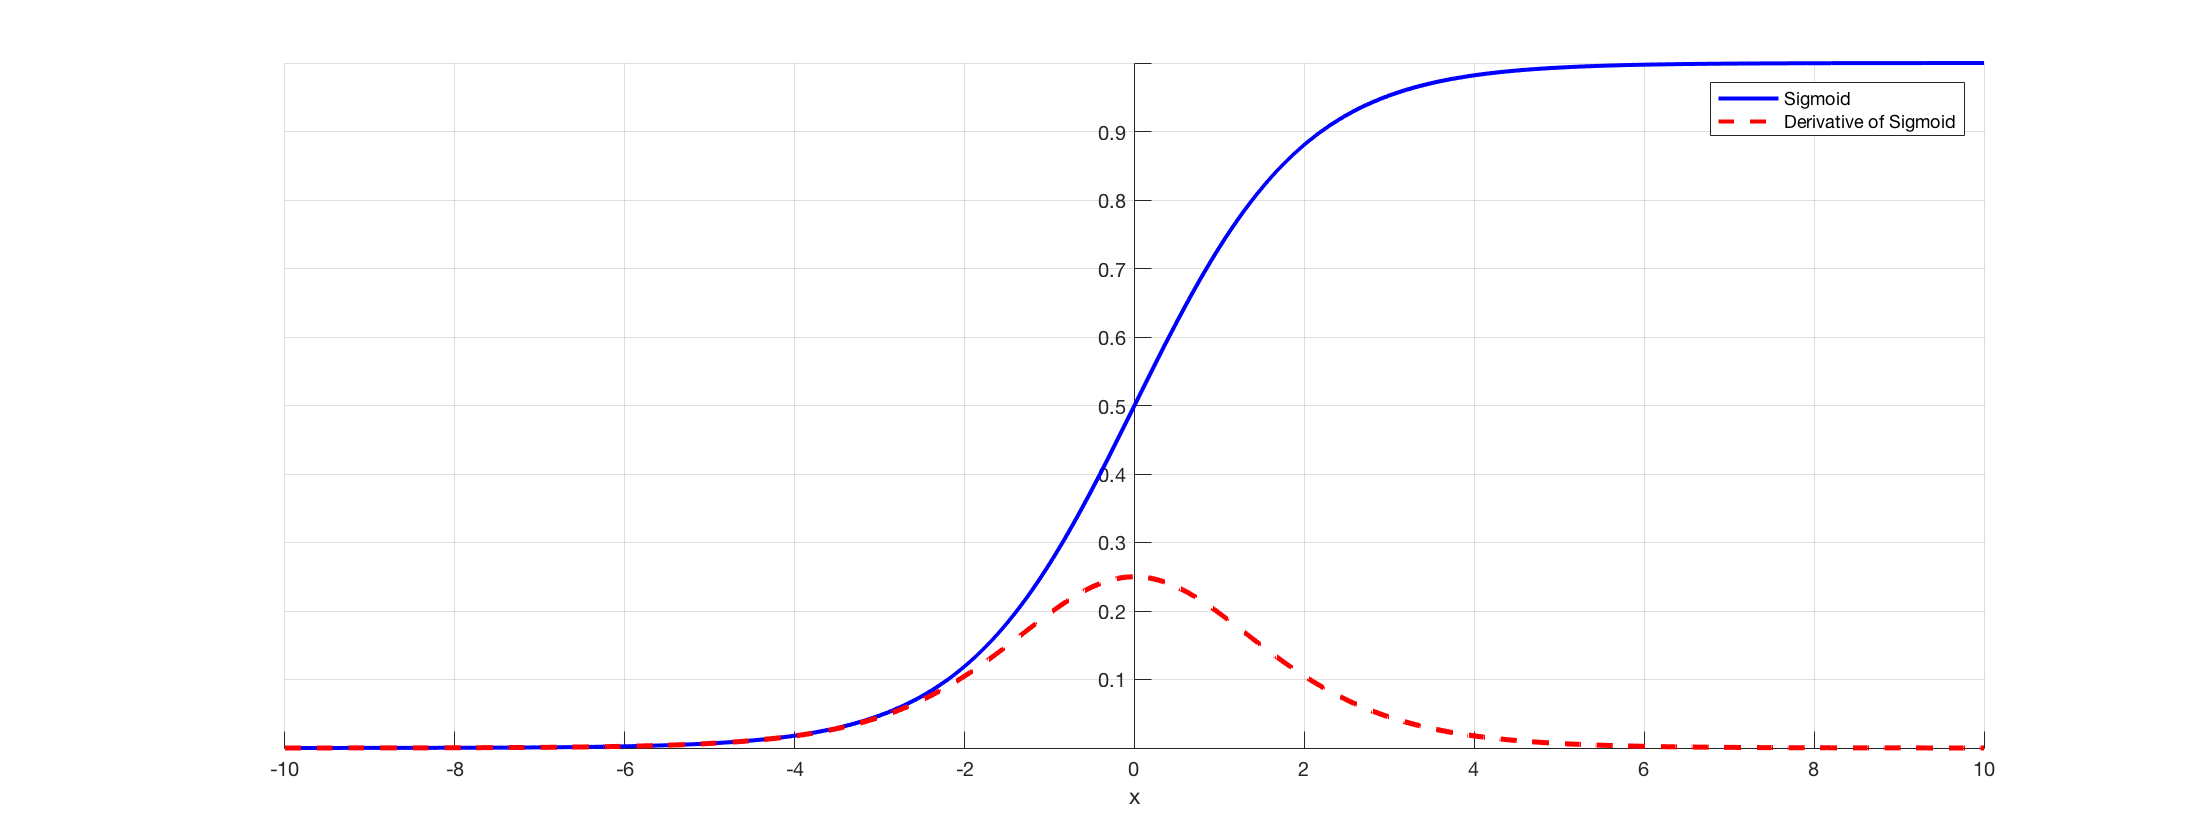
\includegraphics[width=1\textwidth]{sig_der}
                \caption{Plot of the Sigmoid function and its first derivative.}
                \label{fig:sigmoid}
            \end{figure}
            Nevertheless, as the number of layers increases and the network becomes sufficiently deep, the sigmoid suffers from the \textit{vanishing gradient} problem \cite{expvangrads} Fig. \ref{fig:sigmoid}
            due to its derivative being $[0, 0.25]$ bounded. Mainly for this reason it is not widely adopted in practice.

            More in general, the sigmoid lies inside a class of activation functions known as \textit{squashing} i.e. monotonically non-decreasing functions $\varSigma$
            that satisfy
            \begin{equation}
                \lim_{x \to - \infty} \sigma(x) = c, \quad 
                \lim_{x \to \infty} \sigma(x) = 1.
            \end{equation}
            For example, another kind of activation function of this type is the \textit{hyperbolic tangent}, defined as
            \begin{equation}
                \tanh (x)=\frac{\exp \{x\}-\exp \{-x\}}{\exp \{x\}+\exp \{-x\}},
            \end{equation}
            which was find to allow for universal expressivness of the model \cite{hypertanh}. However, as for the sigmoid, squashing functions tend to be prone to vanishing 
            and exploding gradients.

            Nowadays, the most used activation function in neural networks for different applications is the \textit{rectifier linear unit} (ReLU),
            first introduced in \cite{relu} and defined as the positive part of its argument
            \begin{equation}
                \textnormal{ReLU}(x) = \max(0, x),
            \end{equation}
            allows for efficient training and alleviates the exploding gradient problem (having derivative either 0 or 1), introducing only one point of
            non-differentiability. Moreover, it promotes \textit{sparsness} in the network, which is usually beneficial \cite{sparseness}. One problem with ReLUs though 
            is that the neuron's value, that get pushed to a big negative number, might stay stucked in 0 for essentially all inputs, in a so called \textit{dead state}.
            If many neurons in the network die this can afflict the model capacity and can be seen as a form of vanishing gradient problem. To overcome this problem,
            a slighlty different activation functions can be used, called \textit{leaky ReLU}:
            \begin{equation}
                \operatorname{Leaky ReLU}(x)=\left\{\begin{array}{ll}
                    x & \text { if } x \geq 0 \\
                    \alpha x & \text { otherwise },
                    \end{array}\right.
            \end{equation}
            where $\alpha > 0$ is a user-defined constant usually set to small values such as 0.01. Even if this solutions solves the dying neurons problem, it does
            affect the sparseness property of ReLUs.
            
            By definition, the mean of ouput values from a ReLU is always positive. \textit{Exponential linear unit} (ELU) try to normalize their inputs:
            \begin{equation}
                \label{elu}
                \operatorname{ELU}(x)\left\{\begin{array}{ll}
                    x & \text { if } x \geq 0 \\
                    \alpha(\exp \{x\}-1) & \text { otherwise },
                    \end{array}\right.
            \end{equation}
            saturating negative values at a user-defined value $- \alpha$ which is usually set to 1. Conversly to ReLU and LeakyReLUs, the derivative is continuous
            therefore the function is smooth and for the negative values is defined as $ELU(x) + \alpha$.

            Finally, one more recent activation function which gained a lot of attention is the \textit{Swish} function:
            \begin{equation}
                \operatorname{swish}(x)= \operatorname{sigmoid}(x) * x,
            \end{equation}
            
            \begin{figure}[hb!]
                \centering
                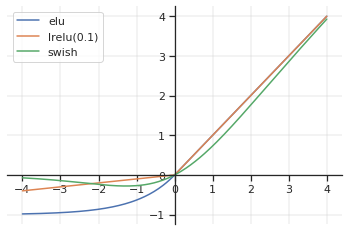
\includegraphics[scale=0.50]{afunctions}
                \caption{ELU, LeakyReLU($\alpha=0.1$) and Swish functions plotted together. It can be seen that they mostly differ for negative values whereas behaving very similar to ReLU for positive arguments.}
                \label{fig:afuncs}
            \end{figure}
            which again does look like another approximation of a ReLU Fig. \ref{fig:afuncs}, but in this case it manages in not loosing any useful property. Indeed, since
            it also saturates at 0 for negative values, it allows for sparsity and being smooth around 0 it helps reducing dying neurons. Lastly, around 0 negative 
            values are kind of preserved which may still be relevant to patterns in the underlying data.
            Swish function proved to consistently match if not outperform ReLU networks in different domains \cite{swish}, and more recent studies showed how this function
            can also help in training more \textit{robust} networks \cite{smooth_adversarial_training}.

            Along with this list of more 'traditional' activation functions, which we will call \textit{fixed} activation functions, there is a whole branch of
            more sophisticated solutions, where the idea is to \textit{learn} the function's optimal shape employing suitable parametric functions. 
            Such functions can then be trained together with other weights of the net using backpropagation and gradient descent. Moreover, following the terminology
            introduced in \cite{kafnets} we can again distinguish between two classes of this learnable activation functions: the so-called
            \textit{parametric activation functions} and \textit{Non-parametric activation functions}. The former being usually a parametrization of a fixed 
            activation function involving few constant parameters, whereas the latter is called non-parametric due to the number of parameters that can in principle
            grow without a bound and involves more complex shapes. At the end of this chapter we introduce a recently proposed class of non-parametric activation functions,
            called \textit{Kernel-Based Activation Functions} which will then be the main tool used in the following chapters to try to build 
             robust neural networks.    


        \section{CNNs: Convolutional Neural Networks}

            \label{cnns}
            In computer vision, in particular for image processing tasks, we can make the assumption that the input to the model will be an image. 
            How well do feedforward neural networks adapt to such inputs? It turns out that we need to introduce several changes in the architecture in order to expect 
            them to work properly. Take for example the famous dataset \textit{ImageNet} which consists of more than $ 14 $ millions of images,
            all of which made of $ 256 \times 256 \times 3 $ pixels. Every fully connected neuron in the first layer would have $ 256 * 256 * 3 =  196608 $ weights,
            thus for a neural network with $ 1000 $ of such neurons, which is a very small number of units in practice, we would already need to train almost $ 200 $ millions of parameters,
            which requires a lot of resources. Therefore feedforward neural networks do not scale well to bigger images. More importantly, assume our task is to 
            classify an image, from the point of view of such models, if we take an image $x$ and perform a translation to, lets say, the right for few pixels, with high 
            probability it will look like a completely different image from the point of view of the net and will probably be classified differently, even if 
            from our point of view is clearly the same image. In some sense, there is no apparent way in which fully connected neural networks can take advantage of 
            concepts such as \textit{locality} or \textit{translation invariance} that are intrinsic to images.
            
            To circumvent these limitations, researchers have developed a specific architecture targeted for computer vision tasks called \textit{Convolutional Neural Network} (CNN) \cite{cnn}).
            In a standard CNN, every layer is $3$-dimensional $(Width \times Height \times Dept) $ to reflect the fact that we are always dealing with images 
            and each neuron is connected only to a constant number of nearby neurons in the previous layer, shrinking down the number of total weights required.
            Layers can be either \textit{convolutive layers} or \textit{pooling layers} or \textit{fully-connected layers}, the latter being a normal hidden layer.

            A convolutive layer takes in input $W \times H \times C_{in}$ neurons from the previous layer and outputs $W \times H \times C_{out}$ neurons, where $ C_{out}$
            is the number of filters used by the layer. A filter $F$ is a $K \times K \times C_{in}$ matrix of trainable weights, with $K>0$ typically a small integer, which is used to
            compute a 2-dimensional activation map by sliding (convolving) across the width and height of the input. At each slice of input 
            $ \mathbf{x_{ij}} = (x^{1}_{ij}, x^{2}_{ij}, \ldots, x^{C_{in}}_{ij})$ that it touches, it computes the dot product $ F^{T}X_{ij}$
            where $X_{ij}$ is the $K \times K \times C_{in}$ window centered at $\mathbf{x_{ij}}$.
            \begin{figure}[hb!]
                \centering
                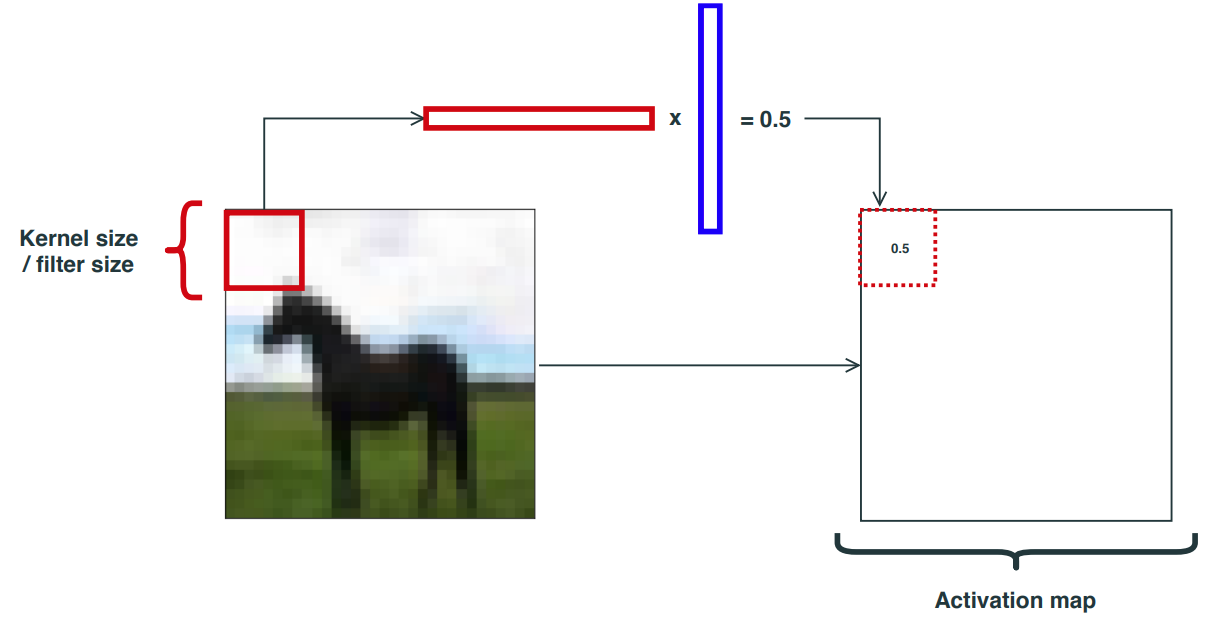
\includegraphics[scale=0.30]{convolution}
                \caption{A convolution that produces the first element of the activation map for the given filter.}
                \label{fig:conv}
            \end{figure}
            Intuitively, through backpropagation we learn filters that are capable of recognizing specific shapes in the image, which we can see as features,
            starting from very concise ones in the early layers to more global ones towards the end layers as the \textit{receptive field} gets larger. 
            Typically, as for normal neural networks, we apply a non-linear transformation after each convolutive layer and by stacking many of these Convolutional
            layers we get a convolutional network.
            
            \begin{figure}[b!]
                \centering
                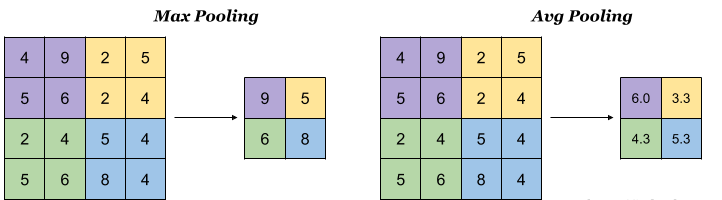
\includegraphics[scale=0.30]{pooling}
                \caption{Max (left) and Average (right) pooling layer with 2x2 window size.}
                \label{fig:pooling}
            \end{figure}
            Going deeper in the network, as we learn global features, it might be convenient to reduce the width and the height dimensions. For this reason CNNs employ pooling layers
            that filters the inputs by some aggregation metric, such as average or max values. Similarly to a convolution, we specify a 
            $ K \times K $ window on which we apply the chosen metric. For example, let $z^{l-1}$ be a $(64,64,12)$ dimensional
            input to a max pooling layer with window size $2\times2$, then, sliding again across width and height of $z^{l-1}$, we take the max value for each
            $ 2 \times 2 $ input patch that we touch. The output will then be a $ (32, 32, 12) $ dimensional vector of max valued neurons Fig. \ref{fig:pooling}. 


            The complete architecture of a textbook CNN is a composition of 2 subarchitectures:
            \begin{itemize}
                \item A sequence of interleaved convolutive and max-pooling layers
                \item A \textit{flatten} layer to reduce the last convolution to a 1-dimensional vector, followed by a sequence of fully connected layers to obtain the final score vector.
            \end{itemize} 
            put together resulting in a  \textit{two-staged architecture}.
            \begin{figure}[h!!]
                \centering
                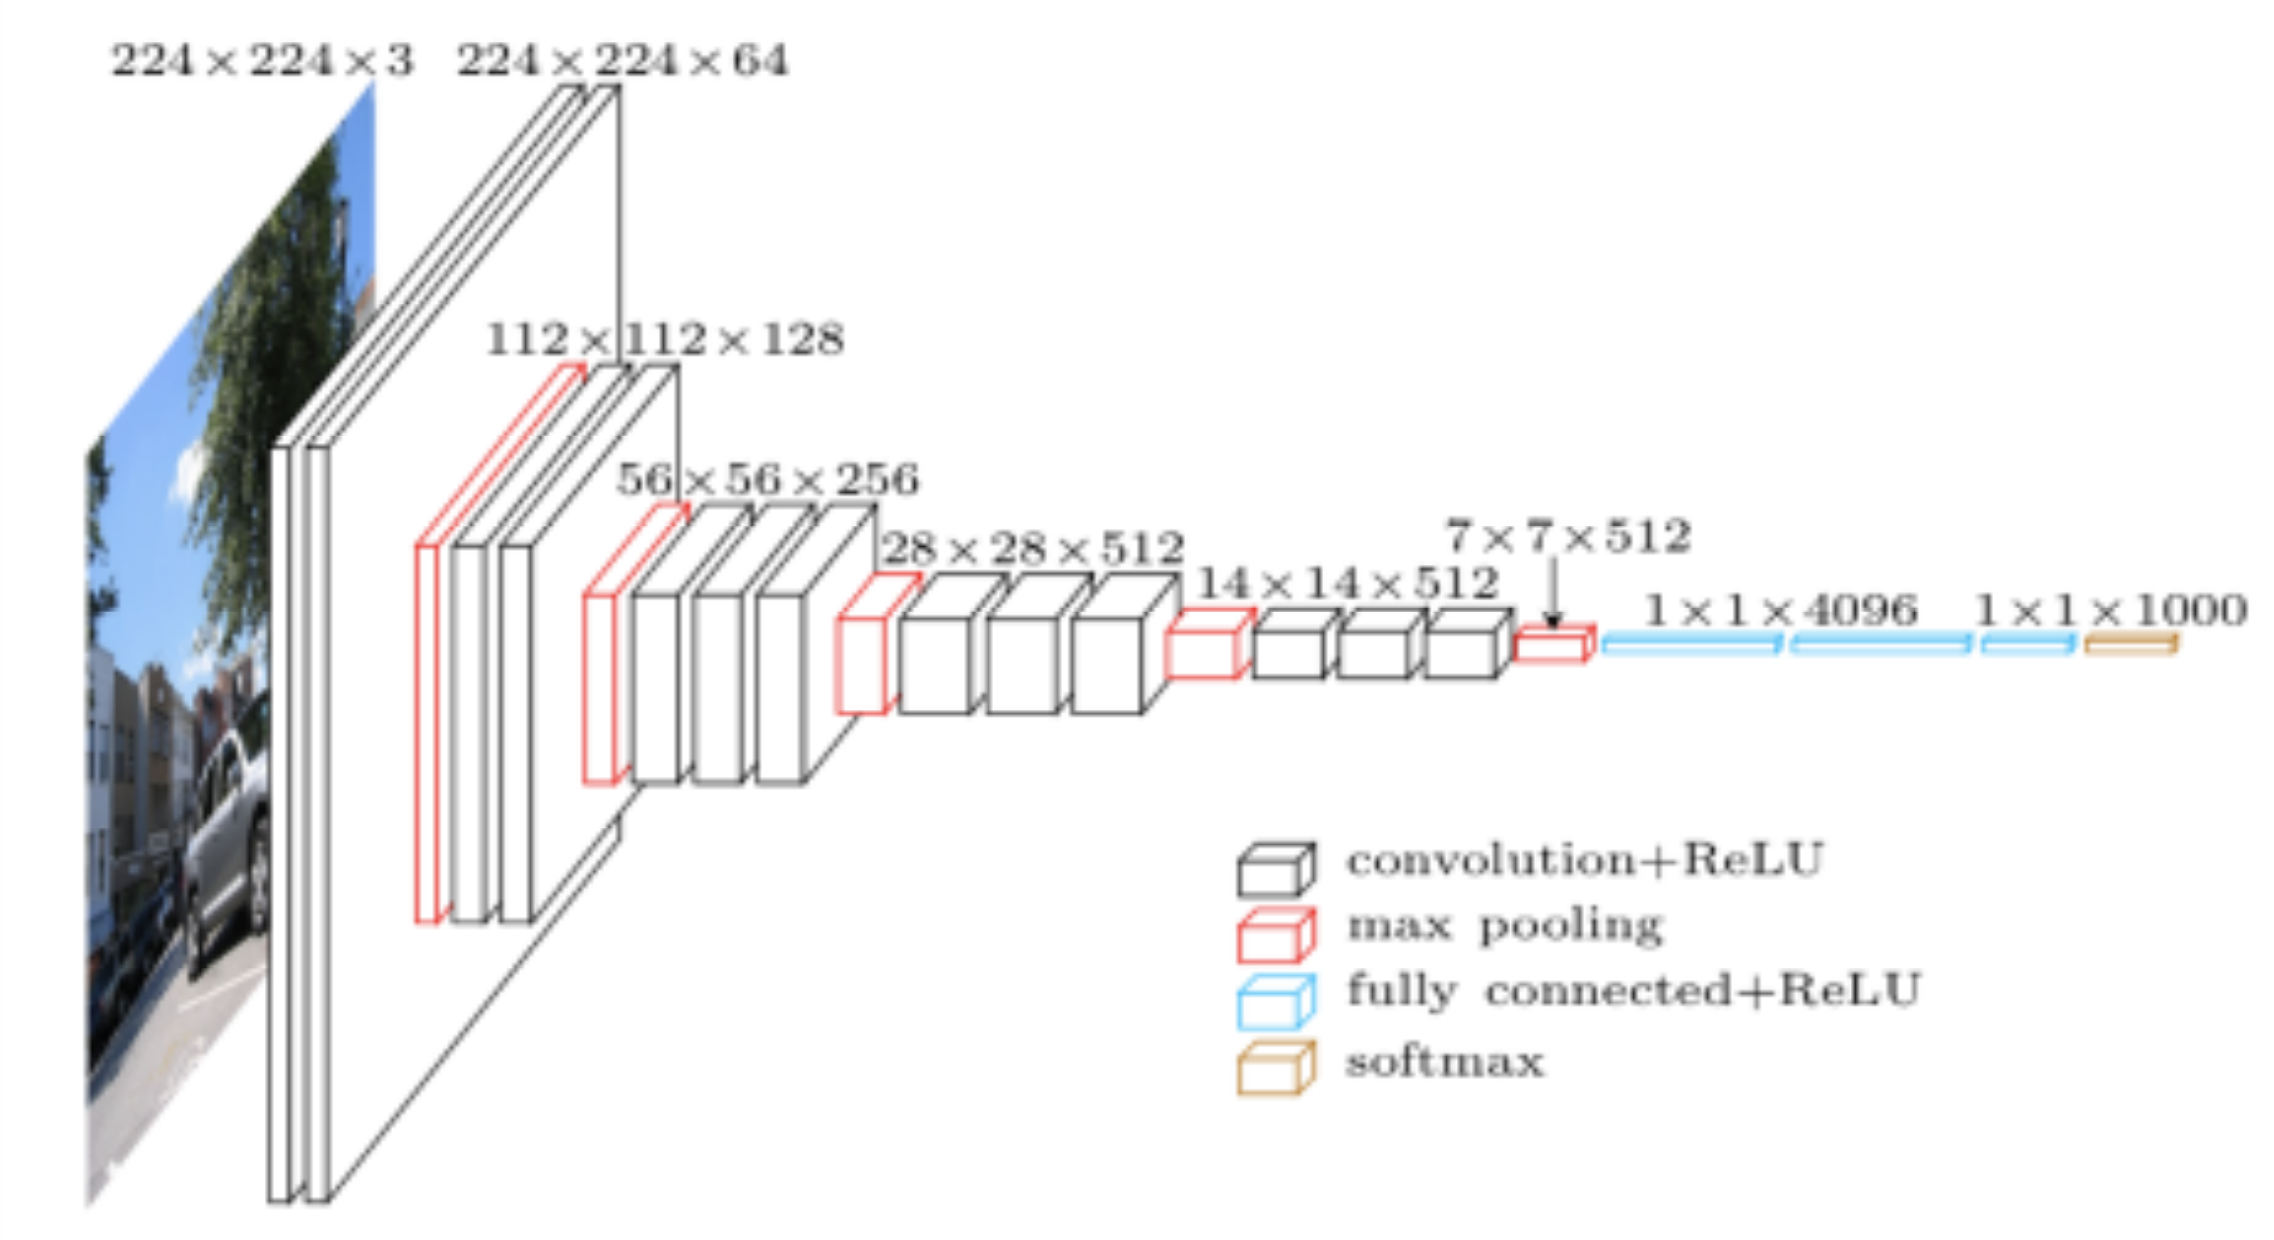
\includegraphics[scale=0.11]{cnnarch}
                \caption{General Architecture of CNN for ImageNet. Source: Kousai S, Understand the architecture of CNN, accessed 20 September 2020, \textit{towardsdatascience.com/understand-the-architecture-of-cnn-90a25e244c7}}
                \label{fig:cnnarch}
            \end{figure}
            
            Even if we can already reach good accuracies with such a basic architecture, modern CNNs employ many smart variations to improve even more the performance,
            as we shall see in the next section. 

        \section{From Neural Networks to Deep Neural Networks}
        \label{dnns}
        Assume to develop a CNN as we have just seen to perform an image classification task. If the built network is sufficiently large, and the chosen dataset limited
        in the number of samples, it might happen that our network will \textit{memorize} the entire trainset instead of learning anything useful from it \cite{overfitting}. The described scenario is an infamous problem in learning theory and goes under the name of \textit{overfitting},
        i.e., instead of trying to learn the ground-truth distribution underlying the data, our model somehow tries to interpolate the training set, 
        resulting in poor generalization capabilities. 
        Early techniques to tackle overfitting involve detection methods such as \textit{early stopping} \textit{earlystopping} 
        or basic prevention methods such as \textit{regularization}\cite{regularization},
        where we try to penalize learning big-valued weights, which are symptoms of overfitting, by carefully adding penalization terms inside the optimization function.

        Despite the fact that the presented techniques are very effective in practice and can help mitigating the problem, they are usually not enough for high performances.
        Another form of regularization can be induced performing \textit{data augmentation} \cite{cnn} which consists in virtually increasing the size of the train set applying
        , for each example in a mini-batch, one or more randomly sampled image transformation such as flipping, cropping, etc. and then train on the resulting augmented
        trainset. Another idea to make the robust against slightly perturbations hence more likely to generalize well is \textit{Dropout} \cite{cnn}.
        Droput extends the idea of data augmentation to the network itself perturbing the hidden layers instead of the inputs by randomly dropping some of the
        neurons. More formally, assume $z^l$ be the output of a generic layer $l$, then applying Dropout to the output means replacing $z^l$ during
        training with:
        \begin{equation}
            \hat{z^l} = z^l \odot m,
        \end{equation}
        where $m$ is a binary vector with entries taken from a Bernoulli distribution with probability $p$. It is important that Dropout gets applied only
        during training whereas at inference time the output of the layer is replaced with its \textit{expected} training value:
        \begin{equation}
            \mathbb{E}[\hat{z^l}] = p \cdot z^l. 
        \end{equation}
        Both data augmentation and Dropout were key components of \textit{AlexNet}, the first CNN to win an image classification
        contest by a big margin \cite{cnn}.

        In 2014, the Oxford's Visual Group realized that they were able to reach better performances than AlexNet by stacking \textit{blocks} of layers instead of many 
        single layers one after the other. In particular, they proposed a block made of multiple convolution layers with $ 3 \times 3 $ kernel size and the same 
        number of filters, followed by a $ 2 \times 2 $ max-pooling, periodically doubling the number of filters for deeper blocks \cite{vgg}. The resulting 
        architecture, known as in literature as \textit{VGG}, was however considerably demanding in terms of resources and this drove researchers to look 
        for solutions that matched the performances whereas decreasing the number of weights. Such goal was achieved soon after with \textit{GoogleNet}
        which made use of two novel modules inside the network: the \textit{inception block} and the \textit{global average pooling} \cite{googlenet}. The former 
        being the first attempt to process in parallel the same input with different levels of granularity, somehow allowing to embed multiple layers within a single
        one Fig. \ref{fig:inception}
        \begin{figure}[h!]
            \centering
            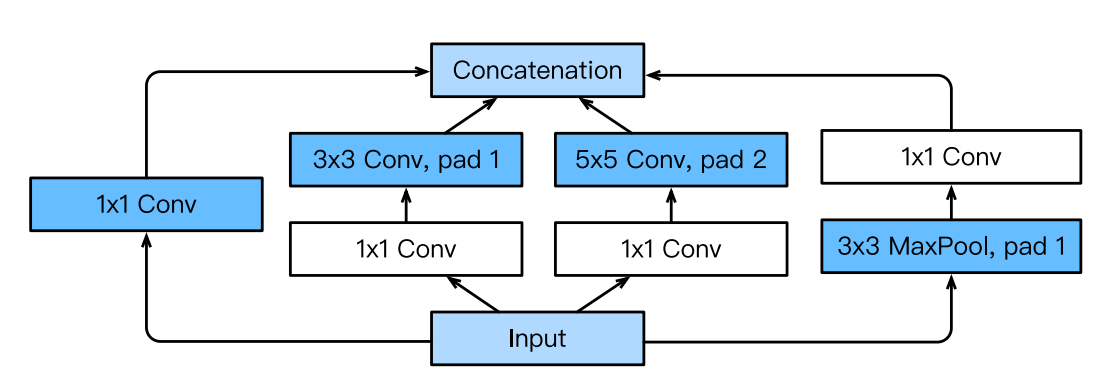
\includegraphics[scale=0.25]{inception}
            \caption{Inception Block overview, $1\times 1$ convolutions are used to reduce the number of filters lowering complexity. Source: Dive into Deep Learning, chapt. 7.4}
            \label{fig:inception}
        \end{figure}
        , and the latter used as a substitute for the flatten layer by taking the average value in each channel and then vectorizing them into a 1-dimensional vector. 
        This last step drastically reduces the number of weights needed in the second stage of the CNN. 
        
        Less than one year later, another breakthrough technique was developed: the \textit{Batch Normalization} (BN), a simple heuristic that 
        allowed to train deep neural nets significantly better  \cite{batchn}. BN works by normalizing and learning to scale the mean and the variance of a layer's output
        in the following way: consider $i_1, i_2, \ldots, i_B$ to be the values of a generic given neuron during a mini-batch. Then with Batch Normalization,
        we first normalize them by:
        \begin{equation}
            i_j = \frac{i_j - \mu}{\sqrt{\sigma^2 + \epsilon}},
        \end{equation}
        with $\mu$ and $\sigma$ being respectively the mean and the variance of the mini-batch values. Then,
        we rescale them by:
        \begin{equation}
            i_j = \alpha i_j + \beta,
        \end{equation}
        where $\alpha$ and $\beta$ are trainable parameters computed with respect to every neuron in the layer.
        Nowadays, it is believed that the reason behind the effectiveness of BN is likely due to its effect on the 
        optimization landscape \cite{bn2}, which gets smoothed, hence the speed-up in convergence and better
        generalization properties.

        Having developed tools that bypass exploding and vanishing gradients, that allow for faster convergence
        and better generalization, one may be tempted in see what happens when we keep stacking more and more layers.
        After all, the intuition we gained from the general trend in CNNs is that the deeper the network, the better
        the learning. However, this belief was not matched by experiments. Indeed, for very deep 
        straightforward neural networks, we are likely to experiment a \textit{degradation} \cite{resnet} of accuracy performances
        which is not caused by overfitting i.e. it leads both to higher test and training error Fig. \ref{fig:degradation}.
        \begin{figure}[h]
            \centering
            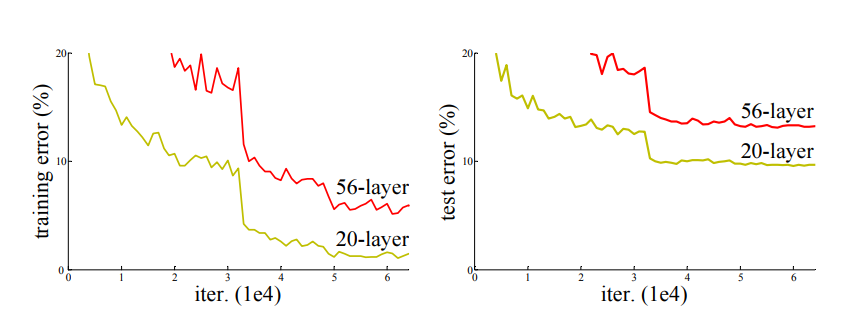
\includegraphics[scale=0.35]{degradation}
            \caption{Source: Deep Residual Learning for Image Recognition}
            \label{fig:degradation}
        \end{figure}
        To approach the problem we can start with the following remark: if we assume a shallow
        network $ \mathcal{F} (x) $ for a given task reaches an accuracy $a$, then by adding identity layers on such network i.e. layers implementing the identity function,
        will result in a deeper network with again accuracy $a$, it can't get much worse.
        Building upon this argument, authors in \cite{resnet} showed that a deep network will rather
        learn a better mapping starting from $ \mathcal{F} (x) + x $ than from $ \mathcal{F} (x) $. 
        For this reason, they introduce the idea of \textit{skipping connections} or \textit{residual connections} where, 
        as the name suggests, we link the input of an earlier layer to the output of a deeper layer, skipping
        over the layers in between Fig. \ref{fig:residual}.
        \begin{figure}[h]
            \centering
            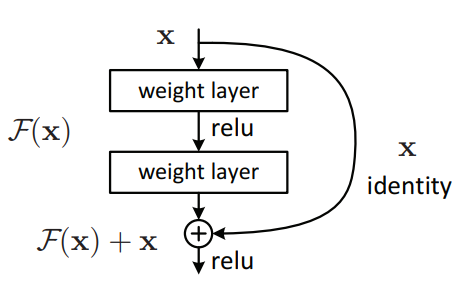
\includegraphics[scale=0.35]{residual}
            \caption{Source: Deep Residual Learning for Image Recognition}
            \label{fig:residual}
        \end{figure} 
        If $x$ has different dimensionality, we can rescale it using a $ 1 \times 1 $ convolution. A neural network 
        that makes use of many residual connections is called \textit{ResNet} Fig. \ref{fig:resnet}. 
        \begin{figure}[h]
            \centering
            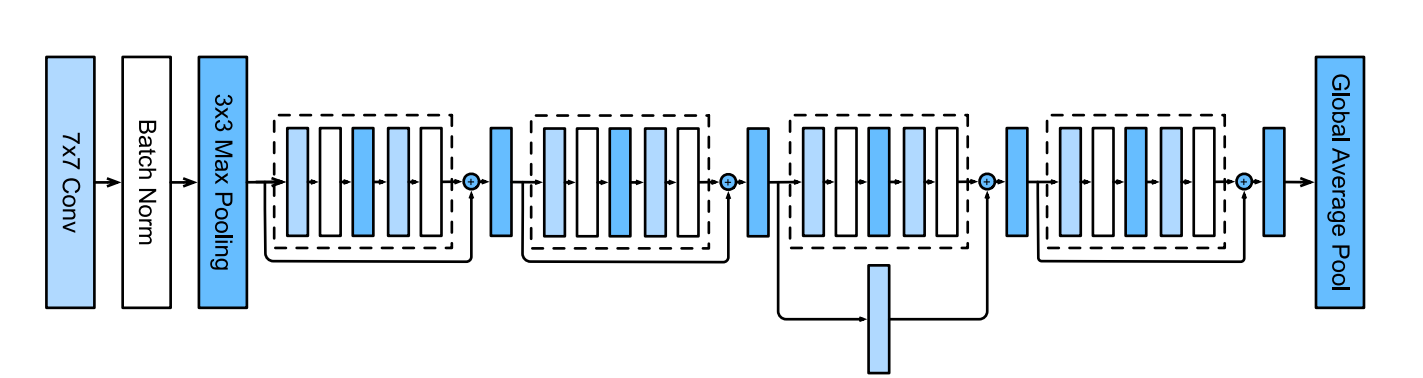
\includegraphics[scale=0.30]{resnet}
            \caption{Source: Dive Deep into Deep Learning}
            \label{fig:resnet}
        \end{figure}

        Thanks to the methodologies introduced so far, we are capable of building non-degenerative CNNs that scale up to hundreds of layers
        and are currently state-of-the-art in many domains.


    \chapter{Adversarial Examples Theory}
    \label{chap:3}

    In recent years, AI-based systems are finding an ever-growing number of applications in the industry, ranging from medical, multimedia, telecommunications, to even military, political and legal sectors. 
    As a consequence of the importance of such systems to the modern world, it is currently reasonable to think that they might become potential threats to the eyes of
    malicious agents such as hackers, business rivals as well as governments, which may seek to circumvent them. For simplicity, we name any of these malicious entities: \textit{adversary}. 
    Inside academia, there is a vast literature on the topic and many attacks and defenses have been devised by researchers towards different types of intelligent systems for both supervised \cite{szegedy2013-intriguing}
    and unsupervised models \cite{unsupervised_adv} with no exception for Neural Networks. Even better, since, as we have seen, DNNs reach best performances among ML systems 
    in many applications, recent research efforts are especially directed in assessing the \textit{robustness} of DNNs. In this thesis we will stick to the same trend.

    In the context of classification, one of the many distinctions that we can make about types of attacks is wether the objective of the attack is to just fool the classifier making it mislabel 
    a given sample $ x $, or targetting the classification towards a specific class $ \hat{y} $ where, given a sample-label pair $ (x, y) $ with $ \hat{y} \neq  y $, our classifier will be tricked in
    believing that the correct classification is indeed $ \hat{y} $. We name this two different scenarios \textit{indiscriminate} and \textit{targeted} attacks respectively. Moreover, despite the fact that the attack is targeted 
    or not, we define three inherently different attacks types against a classifier:
    \begin{itemize}
        \item \textit{Data Poisoning:}
        here the adversarial introduces \textit{poisoned examples} into the data. Poisoned examples can either be mislabeled examples, with the examples correctly belonging to the domain space described
        by the data, or they can be anomalies for the domain. For instance, if data describes birds, a ship should be considered very odd and thus poisoned.
        \item \textit{Reverse Engineering:}
        usually crafted against rule-based classifiers, such attack consists in querying the model to retrieve sensible information about its decision rule or the data on which it was trained.
        \item \textit{Test Time Evasion:}
        as the name suggests, here the attack is performed at test time by a careful \textit{perturbation} of the sample in a way that the transformation is neither human perceptible nor
        easily detected by the system, but as powerful that the classifier's decision now disagrees with a human consensus \cite{goodfellow2014explaining}.
    \end{itemize}
    As shown for the first time in \cite{szegedy2013-intriguing}, DNNs are drastically prone to Test Time Evasion attacks and, more importantly, unaware networks can easily be fooled in a matter of
    few lines of code by anyone who knows the basics of any modern deep learning framework. For this reason, we will dedicate this section to a formal introduction of the problem, and the rest of 
    the thesis in the development of a new approach that aims to improve the resiliency - in jargon, \textit{Robustness} - of Neural Networks against today's Test Time Evasion attacks. 

    \section{Another Optimization problem}
        
        To get a Test Time Evasion attack working, any adversary needs to know the true class of the input he is manipulating. Indeed, the perturbation needs to be done in such a way that 
        the resulting perturbed input will cross the true class decision region, in the output space of the model, to move to another decision region (which is specific to the targeted category in case of a targeted attack).
        However, due to a high number of weights and non-linearities involved in a forward pass, we usually don't know how DNNs actually make their predictions, instead we delegate the job of learning 
        how to make decisions to Gradient Descent during training. Therefore, how does an adversary learn how to craft such untangible yet precise perturbations? Well, he relies again on Gradient Descent, more precisely,
        on back propagation. Recall that, in the previous section, we learned how to compute the gradient $\frac{\partial LS}{\partial w^{l}_{i,j}}$ with respect to any weight $ w^{l}_{i,j} $ of the 
        network, nevertheless, nothing prevents us to push even further automatic differentiation and compute the gradient of the loss with respect to the input $x$ with just as much effort. 
        This quantity will tell us how small changes to the image itself affect the loss function.
        
        Since the goal of the adversary is to make the classifier mislabelling the input, and since we can optimize a function with respect to the input, we can devise an indiscriminate attack by just
        solving the following optimization problem:
        \begin{equation}
            \displaystyle{\max_{\hat{x}} \operatorname{LS}\left(f_{\theta}\left( \hat{x} \right), y\right)},
        \end{equation}
        where $\hat{x}$ is called \textit{adversarial example} and is nothing else that an approximation of the original input $x$. However we also need to characterize the fact that $\hat{x}$ must be very
        close to $x$. In fact, with this settings we could simply transform completly the input to make it equal to another input $x^{\prime}$ which belongs to a different class and would still be
        a valid solution. But this is clearly in contrast with the principle of being an human imperceptible perturbation! Thus denote $\delta \in \mathcal{X}$ to be the perturbation applied
        to the input $\hat{x} = x + \delta $, then the adversary will actually want to solve:
        \begin{equation}
            \label{attackobj}
            \displaystyle{\max_{\delta \in \Delta} \operatorname{LS}\left(f_{\theta}\left( x + \delta \right), y\right)},
        \end{equation} 
        where $\Delta$ denotes the set of any admissible small perturbation. Again, this is something we cannot implement straightaway since it is not clear from a mathematical perspective how to
        explicitly construct the set of all valid small perturbations, even if this is what the adversary is ideally trying to achieve. In practice, what is done is to stick to some mathematical metric such as 
        a specific norm for real vector spaces. For example, an effective metric which allows to fool many NNs, even with super small perturbations is the $L_{\infty}$ norm. The $L_{\infty}$ norm
        for a generic vector $z \in \mathbb{R^d}$ is defined to be:
        \begin{equation}
            \label{linfnorm}
            \|z\|_{\infty}=\max _{i}\left|z_{i}\right|.
        \end{equation}    
        Thus the space of allowed perturbations becomes:
        \begin{equation}
            \Delta = \{ \delta: \|\delta\|_{\infty} \leq \epsilon\},
        \end{equation}
        where $\epsilon$ is the size of the biggest perturbation allowed, i.e. if for example we are dealing with images, any pixel will be $[- \epsilon, \epsilon] $ perturbed and if $\epsilon$
        is chosen sufficiently small, the resulting image will be visually indistinguishable to the original one. However, other norms such as $L_2$ are also very common.

        How do we perform targeted attacks within this framework? Intuitively, the adversary will want to minimize the loss with respect to the targeted class but at the same time, he also wants 
        to be sure that the network will give the smallest confidence to the correct class. This translates into:
        \begin{equation}
            \label{targetedattack}
            \displaystyle{\max_{\delta, \|\delta\|_{\infty} \leq \epsilon }  (\operatorname{LS}(f_{\theta}(x + \delta), y) - \operatorname{LS}(f_{\theta}(x + \delta), y_{target}) )  }.
        \end{equation} 

    \subsection{Fast Gradient Sign Method}
        \label{fgsm}

        For the sake of discussion, we will now see how to actually solve the proposed maximization problems, restricting ourself to indiscriminate attacks, since the same solutions will also
        work painlessly for the case of targeted attacks. 

        In general, the basic idea behind every adversarial attack is to use Gradient Descent to maximize our objective until we converge towards a satisfying solution $\delta^{*}$,
        just as we did when we were training the network. Furthermore, in this case, we also have to take into account the bounds on the perturbation, which can be implemented by a projection  
        to the $[-\epsilon, \epsilon]$ norm-bounded space. In order to maximize loss, we want to adjust delta in the direction of this gradient, i.e., take a step:
        \begin{equation}
            \label{pgd}
            \delta^{t+1} = \delta^t + \alpha \cdot \nabla_{\delta^t} \operatorname{LS}\left(f_{\theta}(x+\delta^t), y\right),
        \end{equation}
        for some step size $\alpha$. Then, we clip $\delta^{t+1}$ to ensure the norm constraints, so in the case of $L_{\infty}$-norm:
        \begin{equation}
            \delta^{t+1} = \operatorname{clip} (L_{\infty}, \delta^{t+1}, [-\epsilon, \epsilon]),
        \end{equation}
        where clipping acts by projecting $\delta^{t+1}$ back to the $\epsilon$-bounded $L_{\infty}$ ball it moved outside.

        Now, if we want to climb the slope of the loss as much as possible we will want to take a very large step size. However, by doing so, we are probably going to stick out the $L_{\infty}$ ball
        and thus our delta will be either be projected to $\epsilon$ or $- \epsilon$ with high probability. Based on this principle, one of the first proposed attack simply considered the following update rule 
        for delta:
        \begin{equation}
            \delta = \epsilon \cdot sign(\nabla_{x} \operatorname{LS}\left(f_{\theta}(x), y\right)),
        \end{equation}
        and is known as the \textit{Fast Gradient Sign Method}(FGSM) \cite{goodfellow2014explaining}. FGSM is a single step attack and works on the assumption that, in a very close neighbourhood of $x$, a DNN can be approximated with the 
        behaviour of a linear model. Consider a simple linear model $ g(x)  = W^Tx $, then $g(x + \delta) = W^Tx + W^T\delta $ and thus, if we want to maximize the effect of the perturbation 
        $ |g(x) - g(x + \delta) | $ under $\|\delta\|_{\infty} \leq \epsilon$ we better define $\delta = \epsilon \cdot sign (W^T)$. Even if the per-component shift is small, the overall shift 
        can increase way more if $x$ is high dimensional.
        
    \subsection{Projected Gradient Descent}
    
        The idea that the effect of any perturbation inside the $\|\delta\|\infty \leq \epsilon$ ball can be approximated, if not upper-bounded, by taking the perturbation at the boundary which
        is given by the direction where the loss is most increasing might be a little too strong as an assumption. Indeed, as previously seen, the optimization landscape is often extremely
        non-linear, even for very small neighbourhoods, thus, if we want stronger attacks, we likely want to consider better methods at maximizing the loss function than a single projected gradient step.

        A more effective and natural approach comes from iterating \ref{pgd} many times with small step sizes and projecting back whenever needed. The general algorithm is called \textit{Projected Gradient
        Descent} (PGD)\cite{madry_adv_training}:


            \begin{algorithmic}[0]
            \Procedure{PGD}{$\alpha, \epsilon$}
            \State $\delta \gets 0$
            \For{$i\gets 1, n$}
            \State $\delta \gets \delta + \alpha \cdot \nabla_{\delta} \operatorname{LS}\left(f_{\theta}(x+\delta), y\right)$
            \State $\delta \gets \mathcal{P}(\delta) $
            \EndFor
            \State \textbf{return} $\delta$
            \EndProcedure
            \end{algorithmic}
        Where $\mathcal{P}$ denotes the projection for the specific metric used. Nowadays, PGD, or slighlty variations of it are standard methods when 
        it comes to evaluate the robustness of a network.

        As for Gradient Descent, PGD is still limited by the possibility of getting stuck inside a local maximum of our objective \ref{attackobj}.
        Mitigations of the problem might arise adding random restarts, i.e., running PGD multiple times from randomly picked starting deltas (within our norm restricted ball).
        It is in fact important to note that it is likely that there are local optima which will be found if we start with $\delta = 0$ and that could be avoided with randomization. 
        Conversely, running multiple PGDs increases the runtime by a factor proportional to the number of restarts and it might not be practical in real-world scenarios, especially when it is used
        as a subroutine to train robust models \cite{free_adv_train}.

    \subsection{White, Grey and Black Box Attacks}

        In the aforementioned attacks, various implicit assumptions are made about the knowledge of the adversary. Biggio et al. in \cite{biggio2013security}
        , in alignment with the wider field of modern Cryptography, have advised making such assumptions explicit also for publications concerning the security of ML models. In particular,
        in any of the previously introduced attacks such as FSGM or PGD, we let the adversary the possibility to exploit the gradients and thus the entire model (perhaps with some hyperparameters excluded) 
        to perform the attack. Such a described scenario, where there is full knowledge about the resources and the model of the defender, is known as a \textit{White Box} attack. 
        Moreover, note as this scenario should be the preferred one since it allows us to devise more effective defenses and is actually compliant with the basic principle
        of "not doing security by obscurity".    
        On the contrary, no knowledge of the classifier results in \textit{Black Box} attacks. Several attacks were nevertheless devised even in such conditions \cite{blackbox}. A more realistic 
        scenario though involves the so-called \textit{Grey Box} attacks \cite{carliniattack1}
        where the adversary might have knowledge of the model but it has no direct access to the training set that
        was used to train the classifier and another surrogate classifier is trained using surrogate data.

        
    \section{Defenses}
        
    Although one may be tempted in the quest for a better understanding of the problem of 
    Adversarial Examples to shed some light on profound questions like: 
    why such brittleness of DNNs exists in the first place, what is that it takes to develop environment-resilient intelligent systems, how are adversarial examples and the interpretability problem related to each other \cite{robustness_accuracy}
    and so on, it is undeniable that the security concerns are, from a practical perspective, the most imminent 
    ones, since, as the integration of ML applications becomes more and more present in 
    the modern world, these issues are starting to threaten several sectors. 
    An attack may, for example, fool an autonomous vehicle which is trying to recognize a road sign, 
    cause a drone to falsely target a civilian \cite{aerialveichles}, or grant authentication to illegitimate people for
    entering buildings, systems, etc. . Therefore, is no surprise that, as soon as
    Adversarial Examples were first discovered, researchers started to come up with many different
    ideas on how to defend ML models against adversaries. In the following, we
    are going to briefly describe some of the most promising attempts that were recently made to develop 
    more robust as well as performant DNNs. 

    \subsection{Detection Methods}

            Detection methods usually involve attaching a 'patch' (or detector) to the original network that we
            want to make robust. The overall network then gets trained, on both original and perturbed samples if the detection
            is supervised, and, with some strategy implementation, the detector learns how to spot adversarial examples 
            from normal ones. 

            \begin{figure}[b]
                \centering
                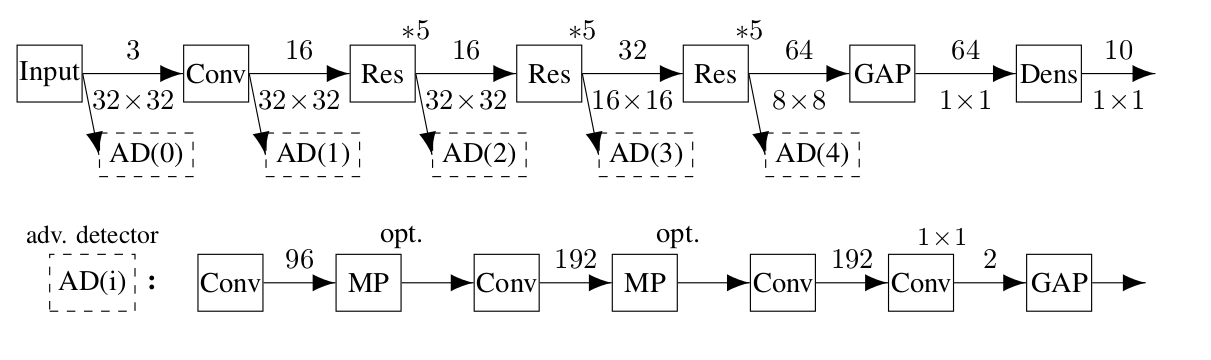
\includegraphics[scale=0.30]{detection}
                \caption{Metzen \textit{et al.} \cite{adv_detect} used a ResNet as original classifier, plus dections is made thanks to many interleaving detectors
                between each residual block. Each detector is implemented as a DNN that learns how to spot the presence
                of an attack by looking at the activations layer's distributions during training.}
                \label{fig:detection}
            \end{figure}

            In the case of a supervised detection mechanism, we want to augment our data with labelled samples crafted with known
            attacks and build a binary classifier which is able to distinguish between vanilla and altered inputs. The key-point here is then to test such a classifier on new, previously unseen attacks and check how well it adapts.  
            Papernot \textit{et al.} in \cite{grosse2017statistical} and Feinman \textit{et al.} in \cite{feinman2017detecting}
            developed two sophisticated early versions of such detection type, but both failed to detect ad-hoc \textit{C\&W} \cite{towards_eval_robustness} attacks on CIFAR-10.
            Better results against C\&W were achieved  by Metzen \textit{et al.} \cite{adv_detect}, whose method
            works by feeding DNN layer's activations as features to a detector Fig. \ref{fig:detection}. In particular, in detecting CW on CIFAR-10
            were 81\% TPR and 28\% of FPR. However they reported that they were not able to generalize well 
            to other attacks, which shows a limitation of their method (or even to any supervised detection?), 
            that is, to likely overfit on the attacks used for training \cite{carliniattack1}.

            In literature, as well as supervised detection mechanisms, there have been also many 
            detection classifiers which were not trained on adversarial examples, thus performing sort-of unsupervised detection.
            They instead rely on an explicit null hypothesis and statistical models to work, such as based on PCA \cite{hendrycks2016early}, which again however showed uneffective against C\&W for CIFAR-10, 
            or on analyzing the joint density of a DNN's layer feature vector.
            In particular, based on the latter, recently Miller \textit{er al.} in \cite{miller2018anomaly} managed to develop the current state-of-the-art for detection
            methods as stated in \cite{adv_survey1} The description of such a method is however quite involving and goes beyond the scope of this thesis.
            
            
            
            \subsection{Robust Optimization and Adversarial Training}

                What if we train a DNN such that, together with minimizing the loss we also
                train to minimize the effects of adversarial examples? That is, how do we go and train
                a DNN which performs well on both clean and perturbed inputs? As it turns out, to perform
                such training, we need to solve the following, intuitive, min-max problem:
                \begin{equation}
                    \label{robopt}
                    \underset{\theta}{\operatorname{min}} \frac{1}{|S|} \sum_{x, y \in S} \max _{\delta \in \Delta} \operatorname{LS}\left(f_{\theta}(x+\delta), y\right),
                \end{equation}
                that goes under the name of \textit{Robust Optimization}.
                
                The order of the optimizations is important here. The maximization is inside the minimization, this
                intuitively means that we are training in a way that: even if the adversary knows the 
                parameters of the model $\theta$ and performs his best attack over it, we contrast
                its effects by minimizing the empirical risk on such an attack, as with standard training.
                Moreover, notice that we just learned how to compute strong attacks e.g. with randomized PGD, thus we
                can already go and implement Robust Optimization, which, to be precise, it is mostly referred as \textit{Adversarial
                Training} (AT) when we approximate the solution instead of computing it exactly \cite{adv_survey2}.

                In practice, even if the training is performed employing random PGD to compute the inner maximization,
                i.e., a very specific form of attack, it does generalize well to other attacks \cite{madry_adv_training}, 
                provided that we consider attacks under the same metric. Indeed, there is no real guarantee that AT
                done under, say, $\|\cdot\|_2$ will result in a model also robust against $\|\cdot\|_{\infty}$ based 
                attacks. To achieve defenses against multiple metrics, we need to incorporate multiple attacks under the inner maximization,
                however, as previously discussed, characterizing a priori every possible metric of perturbation seem to be 
                a difficult task, hence the complexity of devising a universal defense mechanism.

                The main drawback with AT, which is so far regarded as the most effective method developed against adversarial
                examples, is its computational demand. Indeed, due to the double optimization that needs to be
                computed for each weight update on each sample, it requires a lot of resources, especially when it comes
                to large networks and large datasets. For this reason, lately, different works tried to tackle the
                problem of speeding-up AT, proposing approximations and variations of it \cite{free_adv_train}\cite{fast_adv_train}.

                
            
            \subsection{Provable Robustness}

            \label{provrob}
            Provable defenses try to theoretically find certificates in distances or probabilities to certify the robustness of DNNs.
            Can \ref{robopt} be exactly solved? Namely, can we find the optimal set of weights such to minimize 
            the error on Adversarial Examples? This is in principle a legitimate question to ask, and several 
            strategies have been proposed, all of which somehow works providing an upper-bound for the inner maximization.
            In this way, defined the threat model, we can make stronger statements about the guarantees for the defense.
            If we rewrite the innner maximization as the following adversarial loss:
            \begin{equation}
                \mathcal{L}_{a d v}=\max _{\sigma \in \Delta}\left\{\max _{i \neq y} f_{\theta}(x)\left(x + \delta\right)_{i}-f_{\theta}(x)\left(x + \delta\right)_{y}\right\},
            \end{equation}
            then, if we are capable to define an always larger certificate $ C(x, f_{\theta}) > \mathcal{L}_{a d v}$ and prove
            \begin{equation}
                C(x, f_{\theta}) < 0
            \end{equation}
            under certain constraints, the we are sure that, under the same constraints, e.g., on the bound of 
            the perturbation, our model will always predict the correct class. Employing this argument,
            [112] transforms the problem into a linear programming problem and [111] derives the certificate using
            semidefinite programming.
            
            Differently, Szegedy \textit{et al.} \cite{szegedy2013-intriguing} pointed out the relation that exists 
            between the so called \textit{Lipischitz Constant} and the sensitivity of the network 
            with respect to input perturbations. Specifically, denote $f_{\theta}(x) = f_{\theta_L}(f_{\theta_{L-1}}(\cdots (f_{\theta_{1}}(x))\cdots)) $
            then the Lipschitz Constant of  $f_{\theta_i}(x)$ with respect to the norm $ \|\cdot\|_p $ is defined to be
            the smallest $L_i$ such that, for any $x, r \in \mathcal{X}$:
            \begin{equation}
                \label{LC}
                \left\|f_{\theta_i}\left(x \right)-f_{\theta_i}\left(x+r\right)\right\|_p \leq L_{i}\|r\|_p .
            \end{equation}
            Notice how $L_i$ by definition is an upperbound for the sensitivity of layer $i$ with respect
            to any perturbation $r$. Following the composition property of the
            Lipschitz Constant, the overall network Lipschitz Constant will be, the smallest $L$ such that:
            \begin{equation}
                \left\|f_{\theta}\left(x \right)-f_{\theta}\left(x+r\right)\right\|_p \leq L\|r\|_p,
            \end{equation}
            where $L=\prod_{i=1}^{L} L_{i}$. It is important to note how this is only an upperbound, thus a conservative
            measure of the possible unstability of the network. For this reason, no conclusion about the existence of 
            Adversarial Examples can be derived even from large Lipischitz Constants. We are however guaranteed 
            that for very small Lipischitz Constants no Adversarial Example will exist. This is the idea behind 
            many regularization techniques that seek to penalize Lipschitz bounds on networks's components as 
            in \cite{lipschitz_train} 

            Many other approaches try to provide certificates such as \textit{Randomized Smoothing}, \textit{estimation of the lower bound} \cite{randomizedsmooth_cert} \cite{lowerbound_cert}
            . However, provable Robustness struggles to scale up to real-world applications
            due to the complexity of computing such bounds that are usually based on generally intractable methods or ad-hoc methods.





    \chapter{Non-Parametric Activation Functions}
    \label{chap:4}
    As anticipated shortly in the section concerning Activation Functions, it is possible to increase the flexibility of a Neural Network replacing a fixed activation function with a parametrized, differentiable, non-linear function.
    These transformations can in fact be trained along with the remaining weights of the network allowing each neuron to model its own optimal shape.

    Scardapane \textit{et al.} in \cite{kafnets} grouped together different works on such activation functions distinguishing, on the high level, between the number of parameters they involve in their formualtions.
    In particular, whenever we add a constant number of weights to a fixed activation function, authors say we are dealing with 'parametric activation functions'. Some examples of this class of functions are: the \textit{Generalized Hyperbolic Tangent} \cite{hypertanh}
    , a parametric Leaky ReLU introuced by He \textit{et al.} \cite{he2015delving} or the more flexible S-shaped Relu (SReLU) \cite{s-shaped}:
    \begin{equation}
        \label{srelu}
        \operatorname{SReLU}(x)=\left\{\begin{array}{ll}
            t^{r}+a^{r}\left(x-t^{r}\right) & \text { if } x \geq t^{r} \\
            x & \text { if } t^{r}>x>t^{l} \\
            t^{l}+a^{l}\left(x-t^{l}\right) & \text { otherwise }
            \end{array}\right.
            ,
    \end{equation}
    parametrized by $\{t^l,a^l,t^r,a^r\}$. Depending on the values assumed by the left ($l$) and right ($r$) parameters, SReLU can assume both convex and non convex shapes.

    What happens if we give to activation functions greater modeling capabilities, what if we allow them to model any continuous segment? This question is instead addressed by the class of 'non-parametric activation functions'. These methods,
    usually introduce a further global hyper-parameter, allowing to balance the number of parameters that can in principle grow without a bound, hence the name.

    In this section, we give an overview of three early proposals, describing the general idea and some of the drawbacks, if any. After that, we focus on a more recent kind of non-trainable activations called kernel-based activation Functions
    (KAFs), highlighting their properties and experimental results.

    \section{Adaptive Piece-Wise Linear Activation Functions}
            Introduced in \cite{agostinelli2014learning}, APL generalize the SReLU \ref{srelu} activation function summing up $S$ parametrized linear segments that are
            learned under the constraint that the resulting function is continuous:
            \begin{equation}
                \operatorname{APL}(x) = max \{0, x\} + \sum_{i=1}^{S} a_{i} \max \left\{0,-x+b_{i}\right\},
            \end{equation}
            where $S$ is a user-defined value and $a_i$s the parameters to learn. APL adds $2S$ new parameters per neuron i.e. introducing a linear number of parameters to the overall network, which is often feasable.
            APL cannot, however, model or approximate all piece-wise linear functions, but only saturating ones. Moreover, APLs introduce $S$ non-differentiable points which may harm backpropagation.
    \section{Spline Activation Functions}
    If we want an activation function capable of interpolating $S$ given points, we can devise the following polynomial interpolation:
    \begin{equation}
        \sigma(x) = \sum_{i=0}^{S} a_{i} x^{i},
    \end{equation}
    where we actually going to learn $S+1$ coefficients to pass through the desired $S$ points. Thus, in theory, we can at least approximate, by means of
    a sufficiently large $S$, any smooth function albeit in practice, due to the global effect that any parameter has on the global shape, such approximation
    is hard. Moreover, $x^i$ can easily grow too much and encounter numerical problems.
    
    Instead of using polynomial interpolation, \cite{saf} proposed the use of \textit{spline interpolation} that results in the so called spline activation functions (SAFs).
    Let $\{ x_1, x_2, \cdots, x_S \}$ be an equally spaced sampling of real values, symmetric to the origin and with step size $\Delta x$ and call \textit{knots}
    the corresponding y-valules $\{\operatorname{SAF}(x_i)\}^S_{i=0}$ . Denote $u=\frac{t}{\Delta x}-\left\lfloor\frac{t}{\Delta x}\right\rfloor$ to be the normalized ascissa 
    value between to consecutive knots when the activation is $t$. Finally, we can define SAF at $t$:
    \begin{equation}
        \label{saf}
        \operatorname{SAF}(t)=\mathbf{u}^{T} \mathbf{B} \mathbf{q}_{k},
    \end{equation}
    where $\mathbf{u}=\left[u^{P}, u^{P-1}, \ldots, u^{1}, 1\right]^{T}$, $P$ is a user-defined value (usually chosen to be 3), $\mathbf{q}_{k}$ the vector composed by
    the closest knot to $t$ and the $P$ rightmost neighbors knots and $\mathbf{B} \in \mathbb{R}^{(P+1) \times(P+1)}$ the \textit{spline basis}. Different basis give 
    rise to different interpolation schemes.
    
    Good news with SAFs is that each knot has only a local effect on the overall shape. Therefore, with respect to the initialized knots, their training allows for faster and better convergence
    to the optimal. Moreover, as with polynomial interpolation, SAFs can in principle approximate any smooth function. A drawback, however, 
    comparing to ALF, is that regularization techniques cannot be explicitly implemented.
    \section{Maxout Functions}
    One slightly different non-parametric activation function, is given by the introduction of a whole new layer called \textit{maxout function}. With maxout, we compute $K$ different dot products
    on each neuron and then take the maximum:
    \begin{equation}
        \operatorname{maxout}(x) = \max \{  W_i^Tx + b_i \}_{i=1}^K .
    \end{equation}
    A DNN wich employs maxout functions as non-linearities is called \textit{Maxout Network} \cite{maxout}. As for APL, maxout introduces several points of non-differentiability and usually requires 
    \begin{figure}[!h]
        \centering
        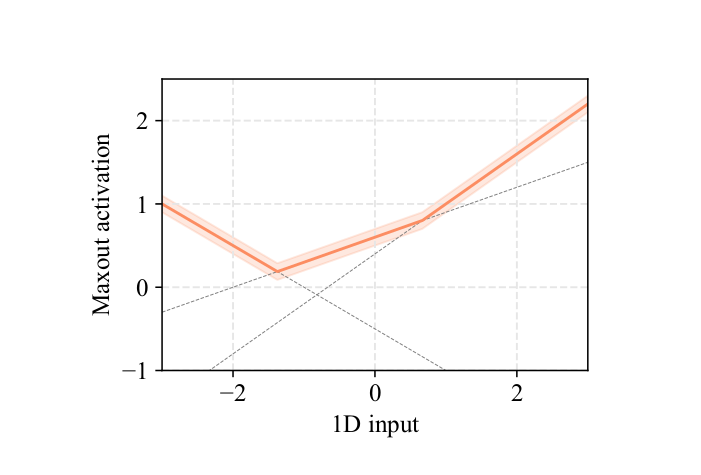
\includegraphics[width=0.6\textwidth]{maxout}
        \caption{A maxout function with a one-dimensional input and K = 3. The
        three linear dot products are shown with light gray, while the max and thus resulting activation is shown
        in shaded red. Source: \cite{kafnets}}
        \label{fig:maxout}
    \end{figure}
    more parameters than previous approaches, as we scale by a factor of $K$ the number of weights inside the net. Furthermore, maxout can only generate convex shapes and 
    we lose the ability of plotting the activation function, except for input up to three-dimensional Fig. \ref{fig:maxout}.
    Different variations aim to solve the smoothness problem for Maxout Networks \cite{maxout1} \cite{maxout2}. 

    \section{Kernel-Based Activation Functions}
    Introduced in \cite{kafnets}, kernel-based activation functions (KAFs) is a class of non-parametric activation functions that leverage kernel expansions to adapt the shape on a per-neuron basis.
    Let $D$ be a user-defined positive integer, then a KAF acting on activation $x \in \mathbb{R} $ has the following form:
    \begin{equation}
        \operatorname{KAF} (x) = \sum_{i=1}^{D} \alpha_{i} \kappa\left(x, d_{i}\right),
    \end{equation}
    where $\{ \alpha_i\}_{i=1}^D $ are the usual parameters to adapt, called \textit{mixing coefficients}, $\kappa \colon \mathbb{R} \times \mathbb{R} \to \mathbb{R}$ is a 1D kernel method.  
    and $\{ d_i\}_{i=1}^D $ the kernel's dictionary elements. Dictionary elements are usually sampled from training data, but in case of activation functions 
    this would tie the size of the expansion $D$ to the specific dataset used. Since generality is preferred, KAFs use fixed dictionary elements by selecting
    $D$ equally spaced points on the x-axis centered at 0 with step size $\Delta$, similary to SAFs. In particular, there is a vast literature on kernel methods with fixed dictionary elements \cite{gaussianproc}.
    A Neural Network that makes use of KAFs is called \textit{Kafnet}.

    To allow for better optimization with Gradient Descent we want the kernel $\kappa(\cdot, \cdot)$ to be positive semi-definite and thus convex, i.e., for any choice of 
    $\{ \alpha_i\}_{i=1}^D $ and $\{ d_i\}_{i=1}^D $ we have:
    \begin{equation}
        \sum_{i=1}^{D} \sum_{j=1}^{D} \alpha_{i} \alpha_{j} \kappa\left(d_{i}, d_{j}\right) \geq 0 .
    \end{equation}
    As for which kernel method one should use, to perform our experiments in the following chapters, we will stick to the original paper and use the 1-dimenstional \textit{Gaussian kernel}:
    \begin{equation}
        \label{gauskaf}
        \kappa\left(x, d_{i}\right)=\exp \left\{-\gamma\left(x-d_{i}\right)^{2}\right\},
    \end{equation}
    where the normalization term $\gamma$ is called \textit{kernel bandwidth} and is empirically chosen to be $ \gamma = \frac{1}{6 \cdot \Delta^2} $.
    The Gaussian kernel is easy to implement using vectorization libraries and quite cheap to compute provided that the dimensions don't grow too large. Moreover, 
    concerning the backward pass, KAFs have pretty straightforward derivatives as well:
    \begin{equation}
        \frac{\partial g(x)}{\partial \alpha_{i}}=\kappa\left(x, d_{i}\right),
    \end{equation}
    \begin{equation}
        \frac{\partial g(x)}{\partial x}=\sum_{i=1}^{D} \alpha_{i} \frac{\partial \kappa\left(x, d_{i}\right)}{\partial x}.
    \end{equation}
    Additionally, employing the Gaussian kernel has two more benefits: first, it allows for locality effects of parameters and second, the resulting (Gaussian) KAF
    is an universal approximator for continuous segments \cite{micchelli2006universal}.

    The mixing coefficients can either be initialized randomly from a normal distribution, giving no direction yet complete freedom in the trend that the modeled shape
    should follow Fig. \ref{fig:rand}, or, on the contrary, we can initialize mixing coefficients such that the KAF will start with an interpolation of any given function $f$
    Fig. \ref{fig:ridge}. Let $\mathbf{t} = (t_1, t_2, \cdots, t_D) $ be the set of values assumed by $f$ when acting on dictionary elements i.e. $\mathbf{t} = (f(d_1), f(d_2), \cdots, f(d_D)) $.
    We can then initialize the mixing coefficients in the following way:
    \begin{equation}
        \mathbf{\alpha} = \left(K  + \epsilon I \right)^{-1} \mathbf{t}
    \end{equation}
    where $K \in \mathbb{R}^{D,D}$ is the kernel matrix with $K_{i,j} = \kappa(d_i, d_j)$ entries, and we add a diagonal term $\epsilon > 0$ to avoid degenerate 
    solutions. To constrain and regularize the learned parameters, contrary to SAFs, KAFs also allow the use of common regularization techniques.
    \begin{figure}
        \centering
        \begin{minipage}{0.45\textwidth}
            \centering
            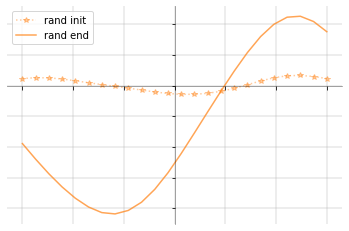
\includegraphics[width=0.9\textwidth]{randridge.png} % first figure itself
            \caption{The shape of a KAF with randomly initialized coefficients is shown in light-starred orange. The final learned shape of the same KAF after 
            training is shown with a continuous orange line. Notice the strong difference between the two functions and how the final one resembles a shifted
            tanh.}
            \label{fig:rand}
        \end{minipage}\hfill
        \begin{minipage}{0.45\textwidth}
            \centering
            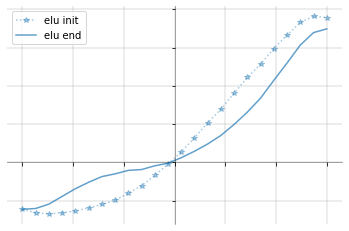
\includegraphics[width=0.9\textwidth]{eluridge.png} % second figure itself
            \caption{The shape of a KAF with coefficients initialized through ridge regression to approximate the ELU function is shown in light-starred blue.
            The final shape after training is shown with a continuous blue line. Notice how the difference between the two is less evident comparing to randomly 
            initialized KAF (left). Both KAFs (left and right) were trained on the same neuron for the \textit{MNIST} dataset using 5 epochs and same overall settings.  }
            \label{fig:ridge}
        \end{minipage}
    \end{figure}
    It is also worth mention that we can improve the flexibility of KAFs by letting the network adapt, along with mixing coefficients, both the dictionary elements
    and the bandwidth. This further level of flexibility can indeed help reach better performances as will be shown in the Evaluation chapter.

    In the original paper authors performed different experiments to assess the performances of the proposed KAFs.
    It turned out that KAFs managed to improve the results obtained with fixed activation functions over several benchmarks ranging from simple datasets 
    like the \textit{Sensorless} dataset  to larger ones such as \textit{SUSY} \cite{susy}, testing on shallow feedforward Neural Networks
    as well as deeper CNNs architectures and for both supervised and unsupervised tasks. A summary of the reported results is given in Table \ref{tab:scardapanekafexp}.  
    
    \begin{table}
        \begin{tabular}{ |p{1.5cm}||p{2cm}|p{1.6cm}|p{2.3cm}|p{2.5cm}|p{2.8cm}|  }
            \hline
            \multicolumn{6}{|c|}{\textit{Scardapane et al. KAF Experiments}} \\
            \hline
            \textbf{Dataset} & \textbf{Design} & \textbf{Metric} & \textbf{Fixed AF}& \textbf{Param. AF} & \textbf{Non-param. AF}\\
            \hline
            \hline
            Sensorless & FNN$^*$  &Accuracy&tanh:99.18\% &PReLU:99.30\% & \underline{ KAF:99.80\% } \\
            \hline
            SUSY&   FNN$^{**} $ &AUC&ReLU:0.8739 & PReLU: 0.8748&Maxout:0.8744 APL:0.8757 \underline{KAF:0.8758} \\
            \hline
            CIFAR10 & CNN$^{***}$ &Accuracy&ELU:78\% & \textit{n.a.} & \underline{ELUKAF:83\%} \\
            \hline
        \end{tabular}
        \caption{Each row summarize the results obtained using different activation functions on a specific task. 
        Underlined entries stand for best result achieved.
        $^*$: feedforward neural networks with 3 hidden layers of 100 neurons are used for fixed or parametric activation functions whilst a single hidden layer is used 
        for KAF activation function.
        $^{**}$: feedforward neural networks with 5 hidden layers and 300 neurons each for fixed or parametric activation functions whilst 2 hidden layers with the same
        number of neurons for non-parametric activation functions \\
        $^{***}$: CNNs made by stacking 5 convolutional blocks, each composed by (a) a convolutive layer with 150 filters, with a
        filter size of 5 × 5 and a stride of 1; (b) a max-pooling operation over 3 × 3
        windows with stride of 2; (c) a dropout layer with probability of 0.25. See the original article for a full description of the architectures, hyperparams and training
        settings.}
        \label{tab:scardapanekafexp}
    \end{table}
       
    
\part{Robustness of Kafnets}

    \chapter{Related Works}
    \label{chap:5}
       
    \section{K-Winners Take All}
    In \cite{kwta}, Xiao \textit{et al.} advocate the use of a $C^0$-discontinuous activation function, called
    \textit{k-Winners-Take-All} (k-WTA) activation, to improve, with no substantial overhead, the robustness of a neural network against gradient-based attacks such as PGD.
    k-WTAs work by acting on the whole layer $\mathbf{y}$, similarly to maxout, but in this case they filter the input retaining the k-largest values and deactivating to 0 the remaining ones.
    More formally, a k-WTA acting on an input vector of neurons $\mathbf{y} \in \mathbb{R}^{n}$ is a function $\phi_k(y) : \mathbb{R}^n \to \mathbb{R}^n$ such that:
    \begin{equation}
        \phi_k(\mathbf{y})_j = \left\{\begin{array}{ll}
            y_{j}, & y_{j} \in\{k \text { largest elements of } \boldsymbol{y}\} \\
            0, & \text { Otherwise. }
            \end{array}\right. 
    \end{equation}
    where $\phi_k(\mathbf{y})_j$ denotes the j-th element of the output. Notice how $\phi_k(\mathbf{y})$ is effectively 
    parametrized by $k$ but it cannot be regarded as a parametric activation function since $k$ is user defined and not
    differentiable. Moreover, since it is likely to have layers with different shapes inside a net, we use the \textit{ratio $\lambda$}
    of the number of neurons of each layer to compute the correct $k$, simply as $k = \lambda \cdot |layer|$.

    K-WTAs foster robustness by making the computation of the gradient $\nabla_x f_{\theta}(x)$ \textit{undefined}.
    Loosely speaking, this is achieved thanks to densely distributed discontinuities in the space of $x$. Indeed, this implies that,
    with very high probability, any perturbation moving $x$ to it's neighbourhood will move over a non-differentiable spot Fig. \ref{fig:kwta}.
    in the adversary objective, making gradient-based search unfeasible. The meticulous reader may at this point start to wonder
    how is thus even possible to perform training with such discontinuous functions. However, it turns out that the gradient 
    with respect to the weights $\nabla_w f_{\theta}(x)$ is discontinuous but in a sparser way, presumably because the parameter 
    space where $w$ leaves is much larger than the input space, allowing the training to succeed. To gain a better understanding
    of what is going on, the paper provides also a theoretical framework in which both the dense discontinuities and the trainability 
    can be explained. Since k-WTAs are only marginally used in the following parts of this thesis, we will not go in the details
    of such proofs.

    \begin{figure}[h]
        \centering
        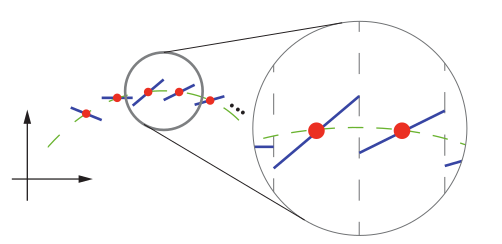
\includegraphics[width=0.6\textwidth]{kwta}
        \caption{A plot of a 1-dimensional k-WTA interpolating a curve. As stressed by the figure, k-WTAs are piece-wise linar functions where points of non-differentiability are 
        very much densely distributed. Any small change in the input results in an abrupt change in the function's value. Source: \cite{kwta}}
        \label{fig:kwta}
    \end{figure}
    
    Authors claim substantial improvements in the robustness of this defense against white-box attacks. Specifically, they were 
    able to evaluate a ResNet-18 against PGD, C\&W and DeepFool \cite{deepfool} attacks, training both classically and with AT \ref{robopt}.
    Using CIFAR10 for the dataset, ResNet-18 with ReLUs achieved 0\% and 43.6\% accuracy under the most effective attack,
    respectively with standard and adversarial training. On the other hand, when k-WTAs were used, the same network improved to
    13.1\% with standard training and 50.7\% with AT.

    In a recent work \cite{carlinikwta}, Carlini \textit{et al.} highlighted fundamentals flaws in the defense that was just claimed for k-WTAs.
    Authors were in fact capable of showing how this method falls within a broader category of attacks, known as gradient-masking
    defense methods \cite{adv_survey2}, which are already known in the literature to be vulnerable.
    It is nevertheless true that, for unadaptive and straightforward implementations of current gradient-based attacks, k-WTAs
    still provide fair protection, especially when the networks is \textit{not} adversarially trained. For this reason, in the following chapters
    we will make use of k-WTAs (for which we give a novel implementation in \textit{TensorFlow2}), as a benchmark for one evaluation.

    \section{Smooth Adversarial Training}
    \label{SAT}

    The current wisdom among researchers, suggests that there probably is a fundamental trade-off between accuracy and robustness that we must deal with
    \cite{freelunch}. That is, improving the resiliency of a model against adversarial examples will almost certainly 
    result in a less accurate model. In particular, whenever an effective technique to improve the robustness is found, it almost always coincides with the method harming
    the model performances \cite{robustness_accuracy}.
    
    To prevent from performance decay, one feasible (but expensive) strategy is to increase the size of the network by making it either deeper and/or wider \cite{scaleintriguing}.
    It seems nevertheless reasonable to believe that there could be other ways that would allows us to build more robust networks without 
    sacrificing in neither accuracy nor resources. That is exactly what was recently reported by Xie \textit{et al.} in \cite{smooth_adversarial_training}, where authors 
    found a way to consistently improve robustness over different tasks, without giving up any other property of the model. Specifically, they found that,
    it is sufficient to prefer and adopt smooth activation functions over non-smooth ones, like the everywhere present ReLUs, to achieve 
    better results in AT straightaway.

    The rationale behind adopting smooth activation functions, i.e., non-linear functions that are continuous in their first derivative, lies in the 
    observation that, during AL, we are computing many times the gradients of the network that are normally required during standard training. Specifically,
    in addition to compute gradients to update the network's parameters, adversarial training also needs gradients computation for generating training 
    adversarial samples. Moreover, the presence of non-differentiable points and abrupt changes in the gradient's values during backpropagation, may 
    prevent from generating sufficiently strong adversarial samples. This particularly holds true in the case of ReLUs, where the gradient lacks of flexibility 
    and gets a severe jump in the origin Fig. \ref{fig:smoothaf}. 

    \begin{figure}[h]
        \centering
        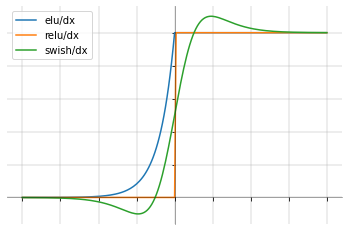
\includegraphics[width=0.45\textwidth]{smothaf.png}
        \caption{Plot of the first derivative for ReLU, ELU and Swish activations. Except for the rectified linear unit, both the ELU and Swish have continuous
        derivative.}
        \label{fig:smoothaf}
    \end{figure}

    To test their hypothesis, Xie et al. evaluated a ResNet50 on ImageNet for different AT runs, by switching activation function after each training. For their experiment,
    parametrized \textit{Softplus}, Swish, \textit{GELU} and ELU were used as smooth activations, whereas ReLU for the baseline. Notice that,
    for the case of ELU, the parameter $\alpha$ \ref{elu} should be set equal to 1 in order to avoid the gradient being undefined at the origin. Compared to the 
    baseline, all smooth activation functions substantially boosted robustness while keeping the accuracy nearly unchanged. In particular, any smooth activation 
    function at least improved robustness by a factor of $5.7\%$. 
    \begin{figure}[t]
        \centering
        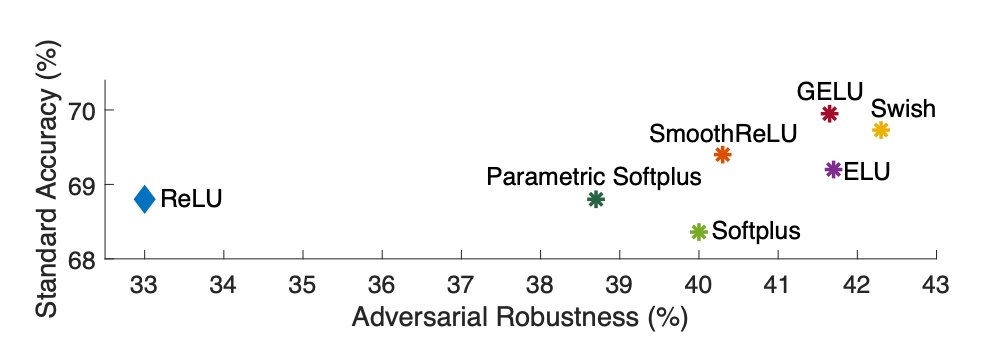
\includegraphics[width=0.75\textwidth]{smoothresults}
        \caption{Compared to ReLU, all smooth activation functions showed a significant increase in robustness
        while some even improved accuracy. In the original work, 2 others smooth activation functions were used, namely 
        SmoothReLU and Softplus. We did not include them since they are not commonly used in practice. Source: \cite{smooth_adversarial_training}}
        \label{fig:smoothresults}
    \end{figure}
    Best results were achieved with Swish, which enabled
    ResNet50 to achieve $42.3\%$ robustness and $69.7\%$ standard accuracy as shown 
    in Fig. \ref{fig:smoothresults}

    To test further the issue with ReLU and generalize the smoothness conjecture, another 
    experiment was made targetting ELUs. As we said, when we set the parameter $\alpha$ to be different to 
    1, the function becomes non-differentiable in the origin, with the gradient
    abruption increasing for larger values of $\alpha$. With no surprise, if we perform the same evaluation with no change in the settings
    except for equipping the network with non-smooth ELUs,
    we observe that the adversarial robustness is highly dependent on the value of $\alpha$. 
    The highest robustness is achieved when the function is smooth while for all other choices of 
    $\alpha$ the robustness monotonically decreases when we gradually approach $\alpha = 2.0$. 
    In particular, with $\alpha$ being $2.0$, robustness drops to $33.2\%$, that is, $7.9\%$ lower than that of smooth ELU. 
    The observed results are consistent with previous conclusions on ReLU: non-smooth activation functions significantly
    weaken adversarial training.

    From a broader perspective, the work on smooth activation functions might
    hints towards the draft of a more general design principle, which is that,
    architectural smoothness might play an essential role in enhancing 
    adversarial robustness, at least for what concerns defenses against 
    gradient-based attacks.

    With a combination of lessons just learned from both Xiao et al. and
    Xie et al., the focus of the following chapters will then be on the evaluation
    of a novel kind of activation functions. Functions that we believe might have 
    , by leveraging, among other properties, strong smoothness
    and flexibility, the potential of surpassing both k-WTAs and Swish 
    for what concerns robustness and, in particular, the trade-off
    between accuracy and robustness. Distinguished activation functions that 
    satisfy such prerequisites are the previously introduced non-parametric 
    kernel-based activation functions (KAFs). 



\chapter{Solution Approach}

    \label{chap:6}
    To test novel architecture components or training techniques with real data, we first need to implement them as software. In our case, 
    we use \textit{Python} \cite{python} programming language and, in particular, experiments are conducted using \textit{TensorFlow2}(TF2)\cite{tf2}, a modern 
    framework for differentiable-programming. In turn, TF2 integrates another famous library, \textit{Keras}, which provides high-level 
    API to build neural networks based models. Specifically, Keras allows to describe customized layers hence it can be used to implement k-WTA and KAF
    activation functions. A working implementation is given in \textit{activationsf.py}.

    \section{KAFs May Be Good Candidates}

        Once the code is done, we can begin and perform some early evaluations. As a first thing, we reasonably chose to test the robustness of simple neural 
        networks and in particular, we can already try to understand if there is any meaningful difference when we change activation functions.

        The light first-developed model is made of few parameters, to conduct quick experiments and perhaps find an initial direction to follow. The network 
        is composed by two convolutional blocks, each of which holding two convolutional layers followed by batch normalization. After those two convolutions we 
        halve the dimensions with a maxPooling and then apply regularization with Dropout. In the first block we use 32 filters, in the second 64, each with window 
        size 3. Finally, a global average pooling is used followed by a fully-connected layer with 128 units which is in charge of computing the output layer.
        The dataset used, and the only one that we will be using for each evaluation, is CIFAR10. The code where such networks are built and trained can be found in 
        \textit{light\_models.ipynb}.

        Respectively, using ReLU, k-WTA and KAFs (with randomly initialized mixing coefficients and D=20) and using Adam optimizer, we obtained 77.96\%, 65.33\%
        and 68.80\% standard accuracy. After that, we are ready to see how such trained nets behave against adversarial examples. Following the settings of 
        \cite{kwta}, a $PGD$ attack is crafted under the $L_{\infty}$ metric, with perturbation size $\epsilon = 0.031$, steps size $0.003$ and 40 random 
        restarts. Importantly, we only attack 1000 random samples taken from the test set, since, due to resource-wise limitations we were not capable of computing 
        the attack on the whole network in a reasonable time and, moreover, because we only wanted to a rough estimate to begin with. To actually implement such attacks we 
        will use the \textit{Adversarial Robustness Toolbox} (ART) from IBM \cite{art}.

        The first results are not really in line with what was expected. In particular, in \cite{kwta} a ResNet18 equipped with ReLUs results in 0\% accuracy 
        against the aforementioned attacks, whereas in our case the net manages, even if with small numbers, to correctly classify 11\% of the 1000 samples 
        attacked. This means that, even if we assume that each of the remaining samples were to be classified wrongly, we would have still classified in the 
        right way the 1.1\% of the test set, in contradiction with the 0\% gained in the original article. However, it plausible that this depends by the model 
        being used, indeed, it is likely that ResNet18 equipped with ReLUs is more prone get fooled by the attack. Despite this inconsistency, k-WTAs on the other 
        hand behave similarly, getting 13,2\% of the samples correctly classified. Another surprise concerns KAFs as well: we managed to reach 15.7\% of accuracy 
        which already a big improvement if we consider k-WTAs were specifically designed to resist gradient-based attacks and still, a straightforward implementation 
        of the KAFs allowed us to overcome them.
        
        Moved by such a result, we decided to go more in-depth with the analysis and look at what is actually happening inside these different implementations of our 
        net when we give adversarial inputs. In particular, we wanted to examine, for each layer, the distributions of the activation values, i.e., the inputs on which activation
        functions act, to see if we could spot any evidence of the observed results. Fig. \ref{fig:actdist13} shows plots for the distributions we obtained when we 
        consider the first neuron of the layer, namely, the fist neuron of the first filter in the case of convolutional layers or the first neuron in the 
        fully-connected layer before classification. Distributions are computed with respect to both perturbed (violet) and non-perturbed (light-green) samples. 

        \begin{figure}[h]
            \centering
            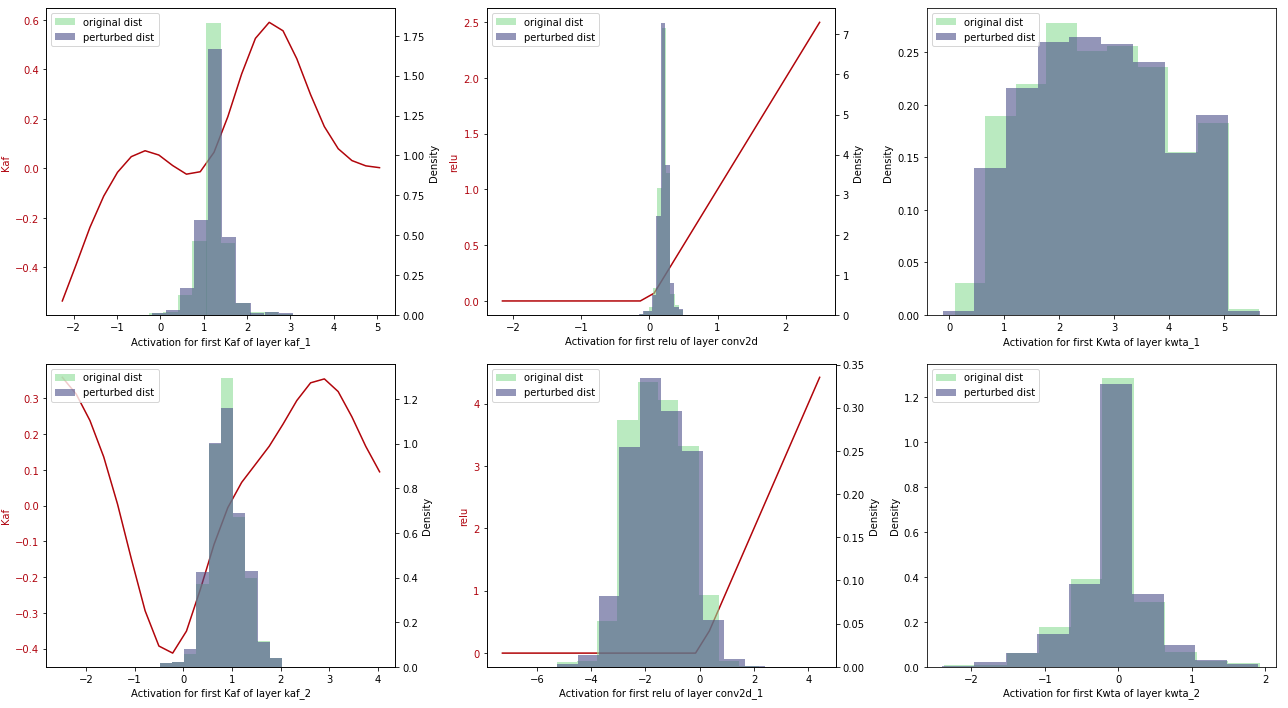
\includegraphics[width=1.1\textwidth]{actdist11.png}
            \label{fig:actdist11}
        \end{figure}
        \begin{figure}[t]
            \centering
            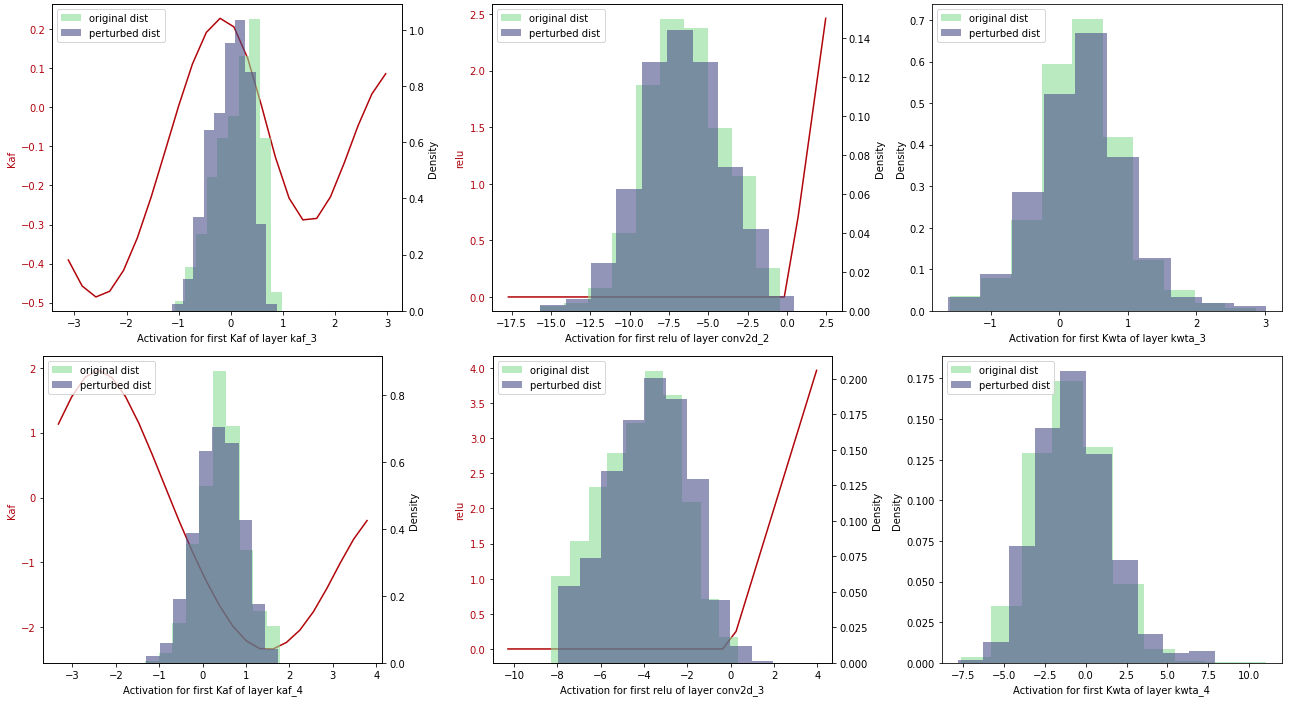
\includegraphics[width=1.1\textwidth]{actdist12.png}
            \label{fig:actdist12}
        \end{figure}
        \begin{figure}[t!]
            \centering
            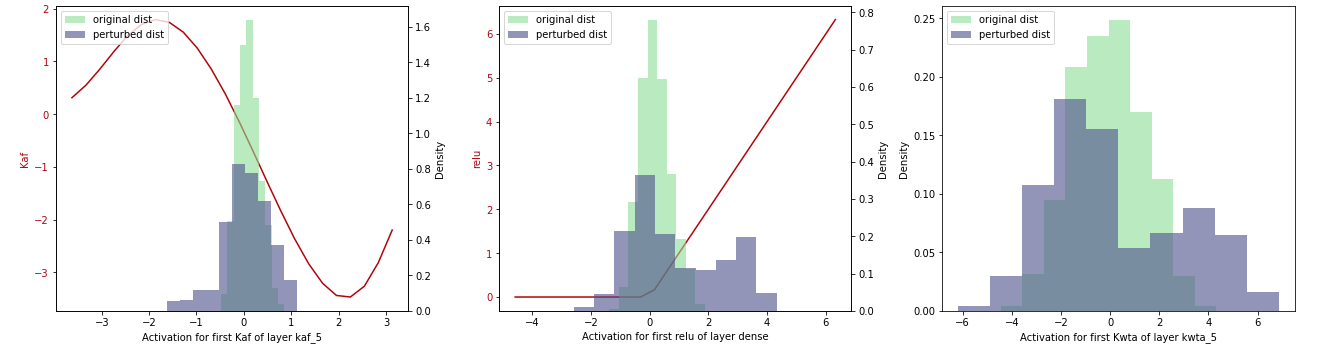
\includegraphics[width=1.1\textwidth]{actdist13.png}
            \caption{Each histogram shows the distribution of the activation values for the first neuron of the first channel, for each layer.
            The distribution colored in violet represents the activations for the batch of perturbed samples while the light-green stands for the 
            distribution of values the neuron gets when we feed the network with original samples. We also plot, when possible, the actual shape of the activation function acting 
            on the neuron with a red line. The effects of the perturbation can be appreciated especially in the last layer where distributions differ the most.}
            \label{fig:actdist13}
        \end{figure}

        The rationale behind these plots is to observe, the more we go deep in the network, how the two distributions, very similar in the initial stages, tend to diverge into two distant distributions.
        This behavior is precisely what we would expect since the networks are making, for the majority of the 1000 samples, different predictions. However, despite 
        the fact that our expectations are confirmed by these histograms, a more careful analysis would also find that the distance in the last KAF layer 
        seem to be smaller in comparison to the distance (between distributions) that we see in the last layer for k-WTA and ReLU. Having said that, it is still plausible 
        that what we concluded might hold true just for the first neuron of the layer while being false in general for the others. For this reason, the next step is 
        to repeat the experiment, this time considering the distribution over more neurons, that is, we consider the average mean for the activations of a given 
        filter, in the case of convolutional layers, or taking the mean of the whole last layer's activations Fig. \ref{fig:actdist23}.

        \begin{figure}[h!]
            \centering
            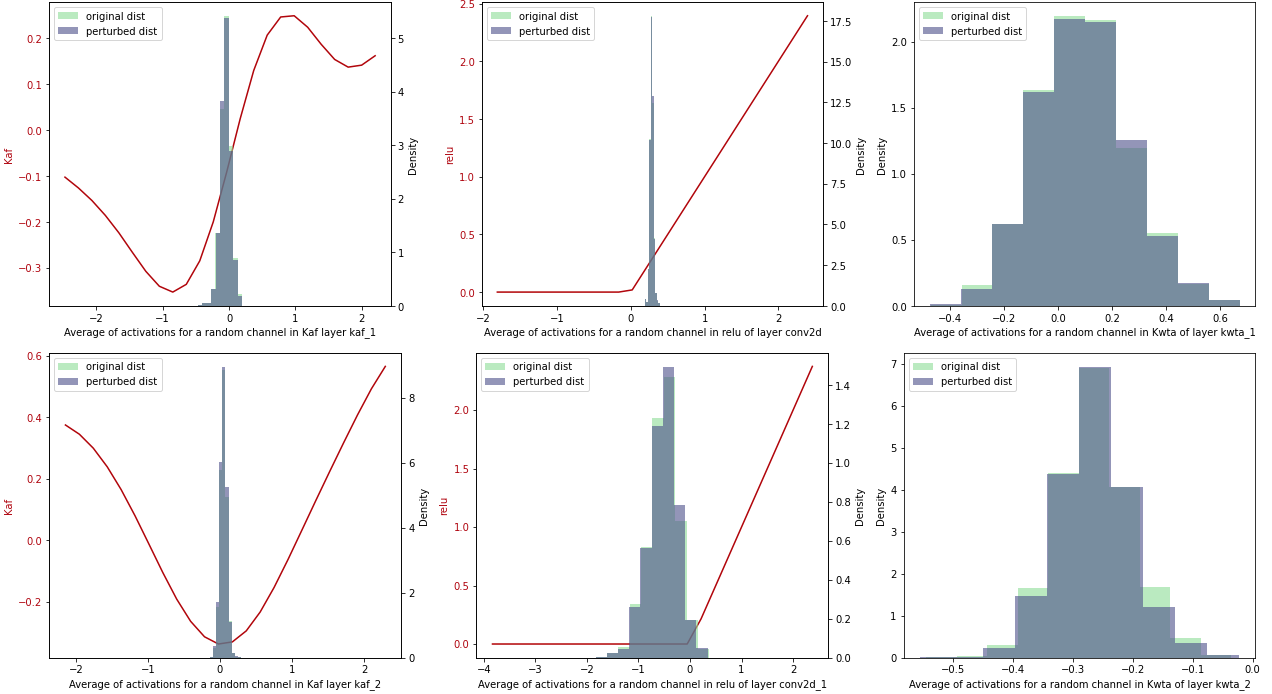
\includegraphics[width=1.1\textwidth]{actdist21.png}
            \label{fig:actdist21}
        \end{figure}
        \begin{figure}[h!]
            \centering
            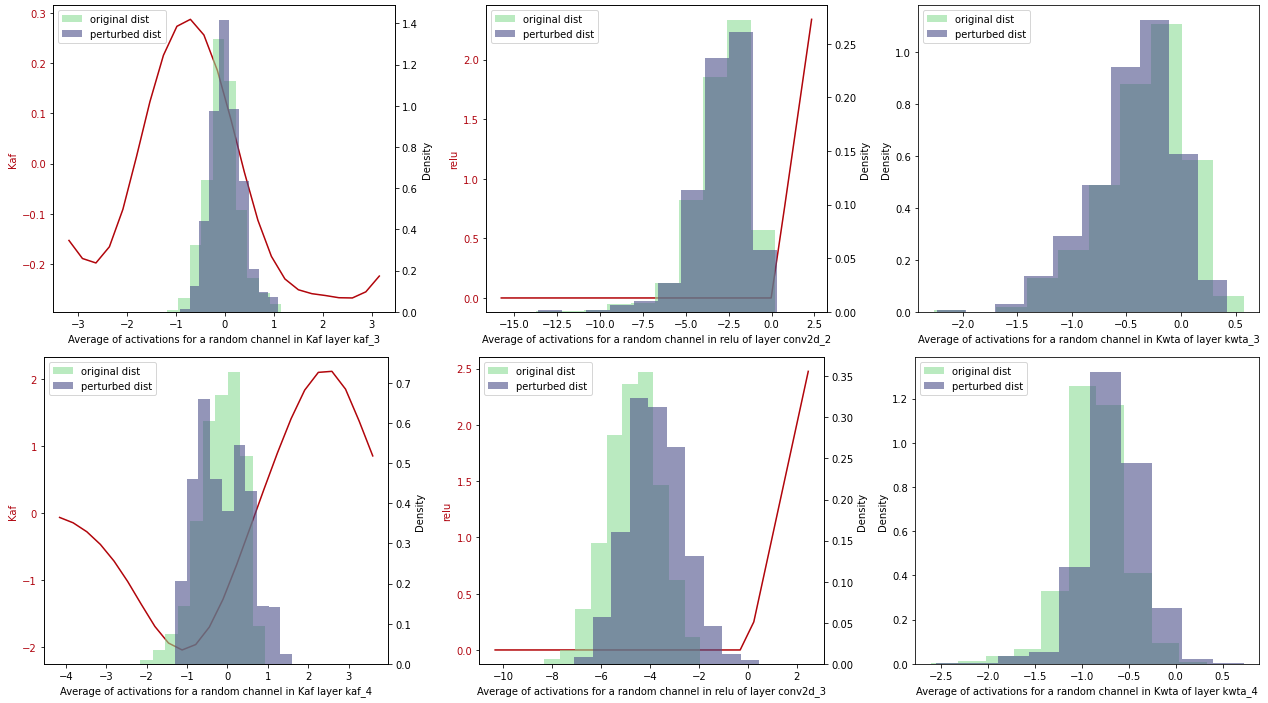
\includegraphics[width=1.1\textwidth]{actdist22.png}
            \label{fig:actdist22}
        \end{figure}
        \begin{figure}[h!]
            \centering
            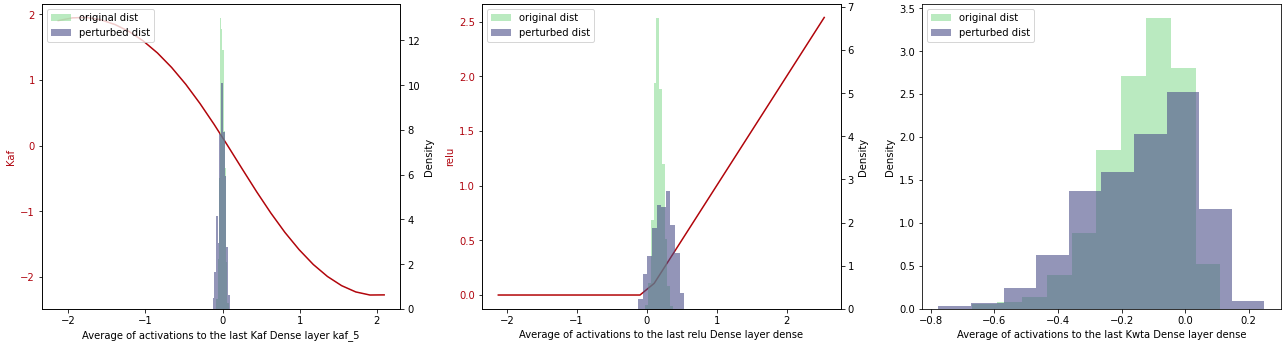
\includegraphics[width=1.1\textwidth]{actdist23.png}
            \caption{Each histogram shows the distribution of the mean value of the activations for a random layer's filter, in the case of a convolutive layer, or 
             for every neurons in the layer, in the case of dense (last) layer. The effects of the perturbation 
             are less visible when the net is equipped with KAF activation functions.}
            \label{fig:actdist23}
        \end{figure}

        
        \newpage
        With more confidence, we can now observe that, what was previously happening in the case of a single neuron is actually happening in general: on average,
        the Kafnet seem to be less prone to big changes within its layers and its output, than when we consider K-WTA, or, in particular, ReLU activation functions.  
        Specifically, if we want to quantify this distance, given $x$ the original input and $x^{\prime}$ its attacked version, we can compute the $L_2$ norm of the difference between perturbed 
        and non-perturbed activations, for each layer. By doing so, and repeating it on many of the attacked inputs, for instance, when considering the first sample and its adversarial pair we get:
        \begin{figure}[h!!]
            \centering
            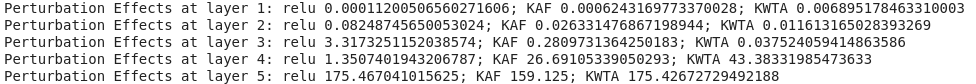
\includegraphics[width=1.0\textwidth]{actdist31}
        \end{figure}
       \newline
        , when considering the second pair:
        \begin{figure}[h!!]
            \centering
            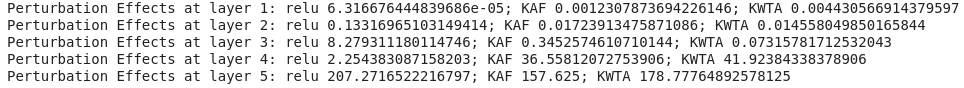
\includegraphics[width=1.0\textwidth]{actdist32}
        \end{figure}
        \newline
        , the 50th pair:
        \begin{figure}[h!!]
            \centering
            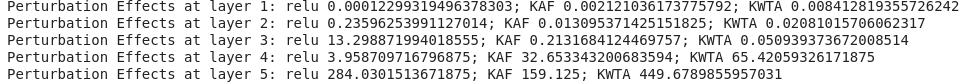
\includegraphics[width=1.0\textwidth]{actdist33}
        \end{figure}
        \newline
        and so on. The Kafnet almost always results in smaller distance norms. The code for reproducing these experiments can be found in \textit{insights\_link\_rob\_activationsf.ipynb}.

        Thanks to in-depth analysis on the architectural statistics we were able, at least from this point of view, to justify why a Kafnet is winning 
        against the other two implementations. Moreover, these results seem to suggest that KAFs, especially when considered together with their flexibility 
        properties, might be good candidates for enhancing robustness through the lens of Robust Optimization. In particular, they seem to fit well when it 
        comes to regularization techniques bounding the effects of perturbations, such as the previously introduced Lipschitz constant regularization \ref{provrob}.
        Even though this regularization technique might appear as the natural approach to follow, it exhibits several difficulties to overcome, such as the lack 
        of efficient and easy to use implementations in current Deep Learning frameworks. Therefore, we opted to approach Robust Optimization with 
        the well-studied method of adversarial training \ref{robopt} and perform the training leveraging also on the smoothness properties of Gaussian KAFs 
        and the previously introduced results linking smoothness and AT together \ref{SAT}.  

    \section{Fast is Better than Free Adversarial Training}
    \label{fbf}
        Adversarial training (AT), can be an expensive procedure to accomplish, and it is not due to the lack of resources but rather to the way we
        implemented it. For example, a textbook implementation of Madry's PGD adversarial training \cite{madry_adv_training}, as for 2019, required 4 days to run over 
        CIFAR10 using a Titan X GPU, and, in order to scale to ImageNet, researchers had to deploy large clusters of GPUs at a scale far beyond the reach of many 
        institutions \cite{free_adv_train}. Consequently, many research has been devoted to improve this computational barrier. For 
        instance, when performing multi-step PGD adversary in the inner maximization, it is possible to cut out redundant calculations during back 
        propagation to gain additional speed-ups \cite{zhang2019defense}. Or, again, instead of updating the network's weights after multiple 
        forward and backwards passes needed to compute the PGD, we could update the weights together with the perturbation $\delta$ at each 
        backward pass of the PGD, hence reducing the overall number of iterations needed to complete the training \cite{free_adv_train}.
        The latter method is know in literature as \textit{Free Adversarial Training} to refer to the apparent relief from the complexity of standard adversarial
        training.
        Nevertheless, even employing these techniques can still result in prohibitive running times.
        
        A recent breakthrough was claimed by Wong \textit{et al.} in their article \textit{Fast is Better than Free: Revisiting Adversarial Training}\cite{fast_adv_train},
        where authors showed they were able to train models that matched state-of-the-art robustness against full-strength PGD attacks, for both CIFAR10
        and ImageNet, in 6 minutes and 12 hours respectively. The proposed method, which allowed them to achieve such results, consists in a mixture of: 
        a clever way for computing the inner maximization in one step, and novel techniques used in efficient 
        training of deep networks, such as \textit{cyclical learning rates} \cite{smith2017cyclical} and mixed-precision arithmetics. The letter being 
        two frequently used key-components in top submissions for image classification competitions like DAWNBench \cite{dawnbench}.
        
        Regarding the method used to approximate the inner maximization, it was used a small variation of the FSGM \ref{fgsm} adversarial training.
        The original FSGM AT works by computing a single step FSGM attack on the mini-batch with step size $\epsilon$ to generate the adversarial sample.
        \newpage
        \begin{algorithmic}[0]
            \Procedure{FGSM\_AT\_ORIGINAL}{$epochs=T$,$dataset\_size=M$,$\epsilon$}
            \For{$t\gets 1, T$} \Comment{For each epoch}
            \For{$i\gets 1, M$} \Comment{For each minibatch}
            \State $\delta \gets 0$
            \State $\delta \gets \delta + \epsilon \cdot sign(\nabla_{\delta} \operatorname{LS}\left(f_{\theta}(x+\delta), y\right))$  \Comment{Perform FGSM}
            \State $\delta \gets \mathcal{P}(\delta) $
            \State $\theta=\theta-\nabla_{\theta} \ell\left(f_{\theta}\left(x_{i}+\delta\right), y_{i}\right)$ \Comment{Update model weights}
            \EndFor
            \EndFor
            \EndProcedure
        \end{algorithmic}
        FSGM AT is generally known to be a weak defense against PGD attacks \cite{physical_adv}.
        Wong \textit{et al.} extended this approach by adding a random initialization of the perturbation 
        $\delta$ (within the allowed space $\Delta$) and by increasing the step size $\alpha$ by a factor of 1.25, making it $\alpha = 1.25 \epsilon$.
        The overall algorithm to adversarially train the model then becomes:
        \begin{algorithmic}[h]
            \Procedure{FGSM\_AT\_Wong}{$epochs=T$,$dataset\_size=M$,$\epsilon$}
            \For{$t\gets 1, T$} \Comment{For each epoch}
            \For{$i\gets 1, M$} \Comment{For each minibatch}
            \State $\delta \gets \mathcal{U}(-\epsilon, \epsilon) $ \Comment{Random init}
            \State $\delta \gets \delta + 1.25\epsilon \cdot sign(\nabla_{\delta} \operatorname{LS}\left(f_{\theta}(x+\delta), y\right))$  \Comment{Perform extended FGSM}
            \State $\delta \gets \mathcal{P}(\delta) $
            \State $\theta=\theta-\nabla_{\theta} \ell\left(f_{\theta}\left(x_{i}+\delta\right), y_{i}\right)$ \Comment{Update model weights}
            \EndFor
            \EndFor
            \EndProcedure
        \end{algorithmic}
        Notice how, for a standard effective AT, that computes adversarial samples via PGD using, say, $m$
        steps, we need to compute $\mathcal{O}\left(mM\right)$ operations per epoch, whereas with $FSGM$ we shrink down 
        to $\mathcal{O}(M)$ operations, i.e., asymptotically equal to number of operations required for standard training.
        Therefore, with only these two small variations to the original FGSM AT, as well as the employment of cyclical learning 
        rates and mixed-precision arithmetic to accelerate convergence, it is possible to devise an 
        adversarial training method, with no significant computational overhead to standard training,
        which achieves leading edge robustness-accuracy trade-offs.
        \newpage
        Moved by the early results obtained on vanilla (i.e. classically trained) Kafnets, and by the 
        feasability of performing strong adversarial trainings, we argue that an evaluation of the robustness of adversarially trained 
        Kafnets is a direction worth taking. More importantly, as previously discussed, the smoothness of network's components, such as 
        activation functions, can additionally boost the resiliency against adversarial examples, and that is precisely the case for Gaussian 
        KAFs. Indeed, recall that the first derivative of a KAF with Gaussian 1D kernel \ref{gauskaf} is given by:
        \begin{equation}
            \frac{\partial g(x)}{\partial x}=\sum_{i=1}^{D} \alpha_{i} \frac{\partial \kappa\left(x, d_{i}\right)}{\partial x},
        \end{equation}
        which is a sum of a finite number of continuous functions $\alpha_{i} \frac{\partial \kappa\left(x, d_{i}\right)}{\partial x}$
        , which makes the whole derivative continuous. Therefore, together with their adaptable nature, we conjecture
        KAFs will improve, with respect to traditional activation functions, both the inner product of adversarial training:
        \begin{equation}
            \delta = \delta + \alpha \cdot sign(\nabla_{\delta}\operatorname{LS}(f_\theta(x + \delta), y)),
        \end{equation}
        in terms of crafting stronger attacks thanks to smoothness, as well as the outer minimization:
        \begin{equation}
            \theta = \theta + \beta \cdot \nabla_{\theta}\operatorname{LS}(f_\theta(x + \delta), y),
        \end{equation}
        where the 'learning' of the attack will benefit from having trainable activation functions, as it happens with standard training
        \ref{tab:scardapanekafexp}.

        This theoretically principled hypothesis on the potential advantages that might come from adversarially train Kafnets 
        needs however an empirical validation. For this reason, the rest of this thesis will be directed into presenting 
        the findings resulted from different experiments we made evaluating the robustness of Kafnets.

       

        


\chapter{Evaluation}
\label{chap:7}
% Goal:
In this chapter, experiments assessing the robustness of Kafnets are discussed. In a comparison with their traditional counterparts, we try to understand 
what is the preferable way to leverage KAFs in this context. If it is by using random initialization of the coefficients, or if we should use them 
to approximate a specific function and use ridge regression initialization. Or again, what happens if we push flexibility even further and we let 
the network train dictionary elements and kernel bandwidths too? Do we gain any improvement? Is there a more advisable architecture for robust 
Kafnets and how well do they perform when we scale to deeper networks? The following sections will cover each of these points. After several evaluations,
we try to interpret the obtained results and highlight why they are or not consistent with our initial hypothesis, what could be the shortcomings of our 
work and, in particular, what are the implications. \par
% Method
To perform each test we make use of the same software environment presented before in \ref{chap:6}, with the addition of \textit{TensorFlow Addons} \cite{tf2},
a library that contains niche functionalities such as the cyclical learning rate technique recommended by Wong \textit{et al.} in \cite{fast_adv_train} to speed-up adversarial training. 
With respect to adversarial training, to the best of our knowledge, there is no implementation available for the extended fast FGSM AT compatible with TF2
at the time of writing. For this reason, we give a working solution in \textit{fbfadvtrain.py} which can reproduce the results
of the original paper. We choose \textit{Google Colab} \cite{colab} for the platform since it provides a built-in installation of the environment plus free access 
to fast GPUs such as NVIDIA Tesla T4, Tesla P100s that can significantly boost the running time. With these settings, each adversarial train 
or attack, the two most expensive operations, 
requires at most 4 hours to complete.

% What
We propose two main experiments, where the only discriminating factor between the 
two is the model architecture. For the first one we are going to employ a VGG-inspired
\ref{dnns} convolutional neural network, whereas for the second one a ResNet20. In
both cases, the task is to devise robust networks for CIFAR10, where robust optimization 
is approached using adversarial learning and specifically we will be using the extended 
FSGM adversarial training discussed above. Following, the resulting trained networks 
are attacked by means of a multi-step PGD attack whose parameters are taken from 
\cite{fast_adv_train}, i.e., with 50 iterations, max perturbation $\epsilon = 8/255$, step size $\alpha = 2/255$, $10$ random restarts
and perturbation metric $\| \cdot \|_{\infty}$. For the optimization algorithm we use 
\textit{Stochastic Gradient Descent } (SGD) \cite{sgd}, as it is the standard choice for 
adversarial training \cite{towards_eval_robustness}. The learning rate is scheduled following
the one-cycle triangular learning rate policy where we let the learning rate linearly 
increase starting from a minimum value in the first epoch to a maximum value in the 
middle of the training and then decrease back with the same ratio until it reaches 
again the minimum value in the last epoch. Additionally, the net can be trained for 
few more epochs were we decrease the learning rate even more from the minimum value 
by another order of magnitude Fig. \ref{fig:oclr}.
\begin{figure}[h]
    \centering
    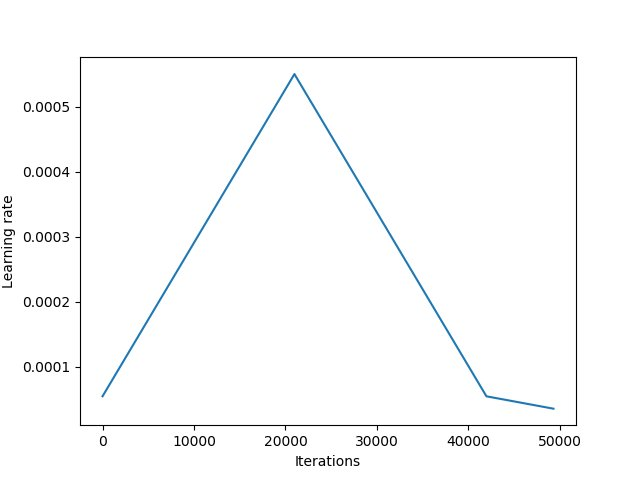
\includegraphics[width=0.50\textwidth]{oclrp}
    \caption{Learning rate evolution during a one-cyclic triangular learning rate schedule.
    Here the minimum value is 0.00005 and a maximum value is 0.0005.}
    \label{fig:oclr}
\end{figure}
The minimum and maximum values are picked through a process called \textit{learning 
rate range finder}(LRF) in which the network gets trained (in our case, adversarially trained)
for few epochs and in the mean time the learning rate is exponentially increased starting from a 
very small value up to a very large one. The overall evolution of the loss 
during this learning rate escalation is then inspected: the minimum value is 
heuristically chosen to be the one from which the loss starts decreasing for the first time 
whereas the maximum value is picked when the loss reaches a plateau Fig. \ref{fig:lrf}
\begin{figure}[h!]
    \centering
    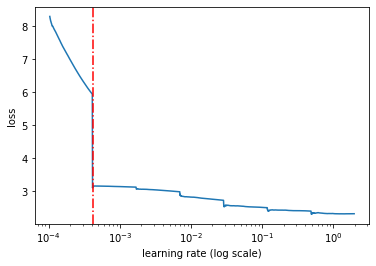
\includegraphics[width=0.50\textwidth]{lrf}
    \caption{Loss evolution plot with respect to exponentially increasing learning rates. The 
    vertical dot-dashed red line denote the learning rate value where the loss has the steepest decrease.
    While the minimum value matches with the smallest learning rate, the maximum one should be picked around
    $10^{-1}$.}
    \label{fig:lrf}
\end{figure}
Different LRF versions are available online, in our case we use one from a public \textit{GitHub} repository\footnote{https://github.com/beringresearch/lrfinder}
since it offers integration with TF2.

Despite the fact that we previously used k-WTAs to show the potential of KAFs, it is worth to 
mention that such comparison was only meaningful for the purpose of our toy experiments, but, in general, 
k-WTAs should not be used as a benchmark for assessing true robustness.
Indeed, as shown in \cite{carlinikwta}, only adding k-WTAs to the network 
is not an effective defense method at all, since they ''make adversarial training worse''.
It turned out that it is actually possible to devise an adaptive, gradient-based attack capable 
of finding many adversarial examples, that brought down the accuracy of the original paper's k-WTA ResNet from 50\% to 16\%. 
Notice how this is not the case for other, standard, activation 
functions: there is currently no gradient-based attack which is known to break a proper adversarially trained network that uses, for instance,
ReLUs activation functions. Therefore, K-WTAs should be considered unsecure. In the following 
sections, we will only be concerned in assessing KAF robustness against well-established counterparts 
like ReLU, that will act as our baseline, or, as previously argued, the preferable ELU and 
Swish smooth activation functions.

    \section{VGG Inspired Architectures Results}
        
        % Architecture
        To begin, we consider a CNN made from convolutional blocks, loosely inspired by the well-known 
        VGG architecture \cite{vgg}. Each block is composed by two convolutional layers with the same 
        number of filters, kernel size 3, interleaved by batch normalization applied before the 
        non-linearities. After convolutions, we apply a $2\times2$ max pooling to reduce dimensionality 
        and dropout for regularization, where the probability for a neuron to get dropped increases
        by 0.05 factor in each application starting from 0.2 in the first one to 0.4 in the last dropout layer.
        We use 3 convolutional blocks with 32 filters in the first one, 64 in the second one and 128 in the third.
        The second stage of the network begins with a 1-dimensional flattening layer applied after the last convolution. 
        Then we fully connect the flattened vector to a 128 neurons dense layer, followed by dropout again,
        and finally the decision layer is another fully connected layer where the number of neurons is equal 
        to the number of classes (10 for CIFAR10) and logits are generated applying a \textit{softmax} application 
        function Fig \ref{fig:vgg}.
        \begin{figure}[h!]
            \centering
            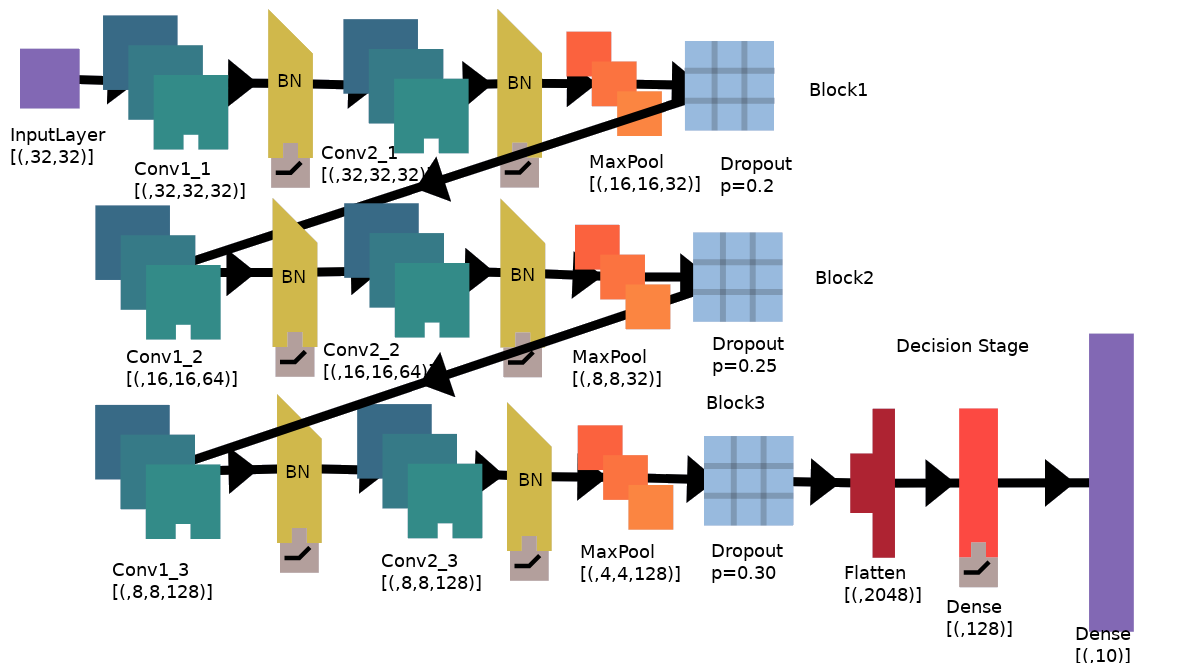
\includegraphics[width=0.85\textwidth]{VGG_inspired_arch}
            \caption{Visualization of the general structure of a VGG inspired CNN. During the experiments
            we will modify the activation function.}
            \label{fig:vgg}
        \end{figure}
        Additionally, we employ \textit{He-uniform} initialization on kernel weights and 
        \textit{$l_2$} regularization on each dense layer with $\lambda$ penality equal to $0.0012$. 
        
        Once the basic structure is built, we only need to plug the specific activation function and test the robustness.
        We start with ReLU, which we consider our baseline. First of all, LRF is run and we find that the min and max learning rate bounds are,
        respectively, 0.0001 and 0.08, and then, we adversarially train the model for 60 epochs. At the end of the training the model with ReLUs achieves 78.1\% of standard accuracy 
        on the test set. Lastly, PGD is performed and the overall accuracy of our network against the perturbed images of the test set is 45.41\%. Therefore, we were able to
        develop a relatively resilient network against full-strength PGD attacks. To be precise, 
        at this point we ran different versions of our PGD by varying the \textit{max\_iter} parameter. It turns out that, for ReLU, just like for 
        the following experiments, the attack converges around the 50th iteration. It is in fact not possible to harm significantly more even if we push 
        the number of iterations up to 150 Fig \ref{fig:pgditers}.
        \begin{figure}[h!]
            \centering
            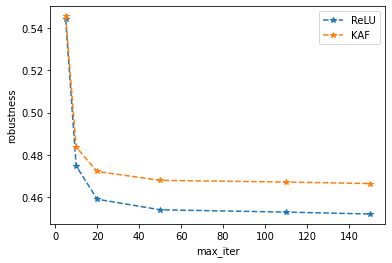
\includegraphics[width=0.50\textwidth]{pgditers.png}
            \caption{Increasing the number of attack iterations inside PGD stops being effective after a certain threshold. With our set-up, 50 iterations are enough to craft an 
            optimal attack. Moreover, notice how the Kafnet improves robustness over the baseline. }
            \label{fig:pgditers}
        \end{figure}
        For this reason we are going to consider only PGD attacks with 50 steps when evaluating.

        We repeat the process equipping the same network with ELU non-linearities. This small change results in a minor improvement over the baseline in terms of robustness, with 45.49\% 
        of the perturbed examples correctly classified. However, the accuracy on clean samples drops to 73.99\%, from an original 78.1\% when using ReLUs. This latter result is 
        apparently in contrast with the claims in \cite{smooth_adversarial_training}, indeed, according the paper, we should have observed an increase in both accuracy and robustness. Nevertheless, this drop could also be explained with a wrong choice of learning rates bounds during LRF. 
        To better understand why this is happening, we test other activation functions, this time using KAFs. In particular, KAFs with randomly initialized mixing 
        coefficients and dictionary size $D=20$ are able to basically match ReLU accuracy, with 77.95\%, and at the same time, to significantly improve robustness achieving 46.80\%
        against our PGD.

        It is reasonable to think that the promising gains that we experiment with KAFs might help us improving or even leveraging the properties of fixed activation functions
        to achieve better scores. Specifically, we build another network where activation functions are KAFs with the same dictionary size as before but, in this case, mixing coefficients
        are ridge initialized to approximate the ELU function. We call such function KAF\_ELU activation function. Evaluating the network with KAF\_ELUs returns 74.93\% accuracy 
        and 45.4\% robustness, i.e., even if slightly better than fixed ELU, these results are still worse than the baseline. Therefore, it is then reasonable to believe that the poor 
        results with ELU and KAF\_ELU are caused by the architecture itself, which is somehow less suitable to ELU-like shapes.

        We are then left to test the activation function which gained best results in \cite{smooth_adversarial_training}: the Swish function. Accordingly to our expectation, with Swish the network 
        boosts in robustness achieving 47.73\%, hence more than 2 points better than with ReLUs, and also improving over KAFs results, making Swish the strongest activation 
        function for this network against PGD, so far. Although, from the standard accuracy perspective, we are still performing slightly worse than ReLU and KAFs, obtaining 
        77\%.

        Similarly to the ELU case, also for Swish we developed a KAF approximation, that we denote as KAF\_Swish. However, if with KAF\_ELU we register close results with respect 
        to the fixed counterpart, with KAF\_Swish activation functions we get greater variations in the two metrics. Indeed, the KAF\_Swish-equipped, adversarially trained 
        network reaches top accuracy with a 78.85\% but worsen the robustness achieving 46.33\%.

        Ultimately, we test another KAF version where kernel bandwidth and dictionary elements are trainable parameters of the network, together with mixing coefficients. In this 
        way, by doubling the number of parameters required for KAFs, we give in principle as freedom as possible in the modelling of an optimal activation function shape. Nevertheless,
        even with this last attempt, the model scores 77.54\% and 46.2\% in accuracy and robustness respectively, positioning these last "moving" KAFs (KAF\_Free), 
        in terms of performances, under the previously used KAF\_Swish. In particular, KAF\_Swish, KAFs and Swish activation functions resulted in best accuracy/robustness trade-offs,
        with Swish achieving strongest robustness and KAF\_Swish strongest accuracy Fig. \ref{fig:accrob1}, Tab. \ref{tab:vggrob}.    
        \begin{figure}[h!]
            \centering
            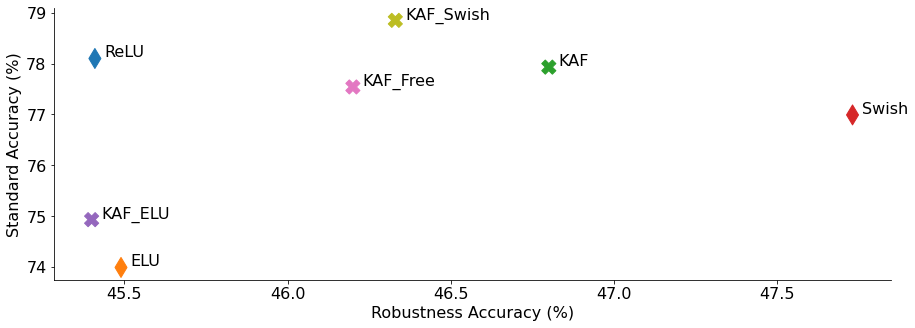
\includegraphics[width=0.8\textwidth]{rob_af.png}
            \caption{Robustness/Accuracy visualization for a VGG-inspired architecture equipped with different activation functions. 
            Fixed activation functions are shown with a thin diamond whereas non-parametric KAFs with a filled x. Swish achieves best robustness and KAFs generally tend 
            to improve both robustness and accuracy with respect to a ReLU baseline.}
            \label{fig:accrob1}
        \end{figure}
        Code to reproduce the experiment and in-depth visualizations on KAF's shapes evolutions are located in \textit{fbf\_training\_kafvgg.ipynb}
        \begin{table}
            \centering
            \begin{tabular}{ |p{2.5cm}||p{3.5cm}|p{1.7cm}|p{2.1cm}|  }
                \hline
                \textbf{Activation} & \textbf{(min\_lr, max\_lr)} & \textbf{Accuracy} & \textbf{Robustness}\\
                \hline
                ReLU & $(0.0001, 0.08)$ & 78.1\% &  45.41\%\\
                ELU & $(0.0001, 0.1)$ &  73.99\% &45.49\%\\
                KAF & $(0.01, 1)$ & \underline{77.93\%}& \underline{46.8\%}\\
                KAF\_ELU & $(0.0001, 0.1)$ & 74.93\%& 45.4\%\\
                Swish & $(0.0001, 0.3)$ & 76.99\% & \textbf{47.73\%}\\
                KAF\_Swish & $(0.0001, 0.8)$ & \textbf{78.85\%}& 46.33\%\\
                KAF\_Free & $(0.01, 2)$ & 77.54\%& 46.2\%\\
                \hline
            \end{tabular}
            \caption{Summary of the results gained from changing activation functions in an 
            adversarially trained VGG network. Bold denotes best result while underline best trade-off.}
            \label{tab:vggrob}
        \end{table}
        
        To what extent these results are accurate? Are we sure that KAFs cannot improve even more robustness?
        Is the Swish function hence the go-to transformation when it comes to robustness? These are all 
        legitimate questions, in fact, somehow our initial hypothesis on the strong properties of KAFs seems
        to be only partially true. From our experiments it emerged that Swish function works better than KAFs
        if our only concern is robustness. However, a couple of things should be highlighted here. First of all, 
        in many cases with KAFs and its variations (KAF\_ELU, ..) we noticed, at the end of adversarial 
        training, that there was still room for learning Fig. \ref{fig:vgghistory} and thus, 60 epochs might as well 
        acted as a limitation in our evaluation process. 
        \begin{figure}[h!]
            \centering
            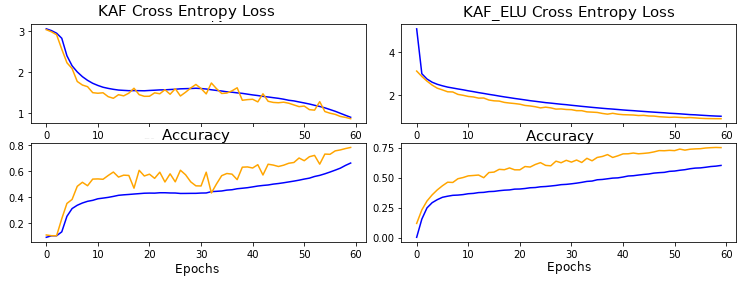
\includegraphics[width=0.8\textwidth]{historyvgg.png}
            \caption{Accuracy and loss evolution during AT. The orange denotes the metric evaluated on the 
            train set while with blue we denote the metric for the test set. In the left the plot for 
            KAF training is shown and in the right for KAF\_ELU. Notice how in both cases there is 
            no sign of convergence at the 60th epoch.}
            \label{fig:vgghistory}
        \end{figure}
        Furthermore, in our designed architecture,
        we made extensive use of max-pooling layers, applying them three times during a forward pass. 
        Even though they are very useful components in a neural network to decrease dimensionality and 
        avoid redundant information \ref{cnns}, it is also true that such layers are non-smooth by construction.
        In fact, they introduce jumps in the gradient computation, acting similarly to the previously 
        discussed k-WTAs. Therefore, our attempt in exploiting the smoothness of novel activation functions 
        might have failed a priori, due to the presence of non-smooth components in our architecture which 
        canceled out our efforts. Notice how this argument could also explain why we had suprsingly poor 
        results with ELUs and their KAF approximation.

        In light of such considerations, we decided to repeat the experiment this time employing another 
        architecture which was free from non-smooth components. A natural choice in this regard, 
        due to its simplicity and great performances was to implement and evaluate a residual neural 
        network (ResNet) \ref{dnns}.  


    \section{Exploding Gradients with KafNets}

        For the implementation in TF2, we follow the architecture described in the original paper by He \textit{et al.} \cite{resnet}.
        In their study, authors design and evaluate two different ResNets, regardless of the number of layers, depending on the dataset used: 
        one for ImageNet and the other for CIFAR10. Since we are using the latter dataset, we are going to stick to that specific ResNet.
        As for VGG, the basic structure of the architecture is a block of convolutions, made of two $3\times3$ convolutions interleaved by BN and non-linearities 
        plus a residual connection between the input to the block and the output of the second convolution. Moreover, we divide the convolutive stage 
        of the network in three sections articulated by their features map dimensionality which are $\{32, 16, 8\}$ respectively. Instead of using 
        max-pooling to reduce the features map size we use strides of $2$ in the first convolution of the block. The number of filters for 
        each section are $\{16, 32, 64\}$ respectively. Before these sections there is another $3\times3$ convolutional layer which halves the input dimension.
        Finally, the network ends with a global average-pooling, a fully-connected layer with 10 units and a softmax.
        In total, the number of layers of such ResNet is given by:
        \begin{equation}
            6n+2,
        \end{equation}
        stacked weighted layers, where $n$ denotes the number of residual blocks in each stage.
        Differently to the previous experiment with VGGs, this time we use the following data augmentation on the training set:
        4 pixels are padded on each side of the image and a $32\times32$ crop is randomly sampled from the resulting image or its horizontal flip.

        To check if we correctly implemented the described network, we try to replicate the results obtained by the authors in the paper for $n=\{3, 9\}$ therefore 
        for a ResNet20 and a deep ResNet56 using the original training settings. The models are trained with a mini-batch size of 128 and for 150 epochs, with a learning rate of $0.1$ and ReLU
        activation functions. At the end of the last epoch, our implementation for ResNet20 returns 91.8\% of standard accuracy which matches the original results. Similarly, when scaling to ResNet56 we get 93.22\% which, even if slightly
        worse than the originally reported 94\%, is still sufficiently accurate. We then managed to have a working implementation for ResNet and we can start our evaluations.  
        
        Since we are mainly concerned in testing the model with other activation functions, we perform a sanity check with KAFs, to make sure that we do not experience drastically 
        changes in the outcome. Therefore we train, with equal settings, a KafResNet20 and a KafResNet56. Surprisingly, if with 20 KAF layers we get a reasonable 90.07\% of standard accuracy, that may be 
        improved by tuning KAF parameters, in the second case, our 56-layered Kafnet is unable to learn anything at all from the data. 
        \begin{figure}[h!]
            \centering
            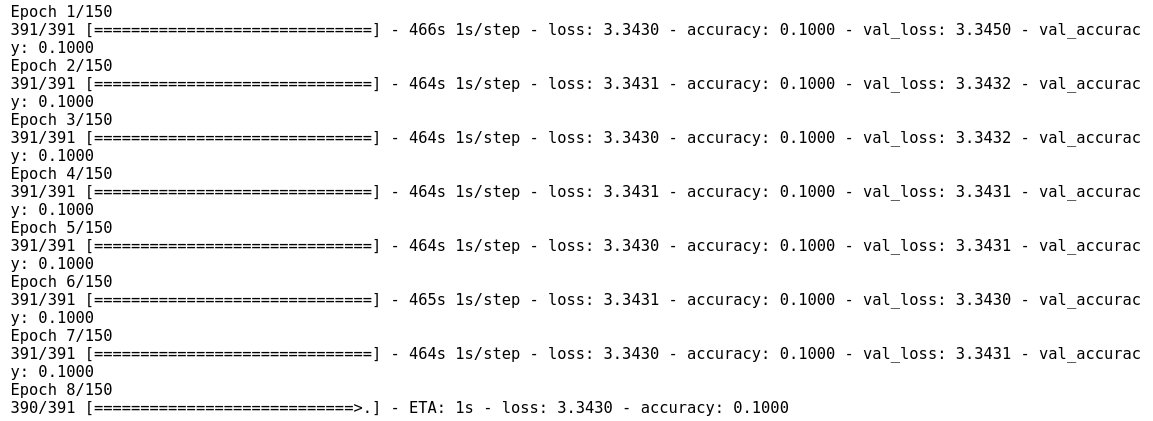
\includegraphics[width=0.8\textwidth]{explgrad.png}
            \caption{}
            \label{fig:explgrad}
        \end{figure} 
        As can be seen from Fig. \ref{fig:explgrad}, after 10 epochs the classification is still performing randomly. Moreover, this trend does not change even if we let the network train longer or if we tune learning rates, KAF parameters 
        or kernel weights initialization. 
        
        Since we know that the overall architecture works correctly when ReLUs are used, the problem needs to be related with the integration of KAFs. Nevertheless, we also know that KafResNet20 works flawlessly and thus,
        this issue only arise with the application of KAFs in deep scenarios. For this reason, we argue that the behavior we are facing is probably due to an issue with gradients updates in the network such as 
        vanishing or exploding gradients.

        To test if this is indeed the case, we log and analyze the distribution of the \textit{Euclidean} norm for each weight, gradient pair inside the model during the first few epochs of the training. The analysis is carried out 
        on every developed network, i.e., for both ResNet20 and ResNet56 when equipped with ReLU or KAF activation functions. To mitigate the running time, we only log the first epoch for KafResNet56 and the first 4 for the remaining architectures.
        After logging the inner statistics, we compare each model with their graphical visualization of the
        evolution of weights and gradients values. The idea is that, in the presence of vanishing or exploding gradients, we should be able to graphically spot where the problem happens, by means of macro variations in the 
        KafResNet56 plots. All the visualization are made using the \textit{TensorBoard} tool.
        
        To showcase the effects of a potential gradient issue, we inspect three different areas of the network: the early layers, some of the middle layers, and the very last layers. In fact, 
        wether we are dealing with exploding or vanishing gradients it would eventually become clear in the early stages of the network, however, since our goal is to understand where the phenomenon starts to emerge
        we need to inspect also the remaining layers. 
        
        As can be seen analyzing the first convolution and the first KAF Fig. \ref{fig:gradkaf1} \ref{fig:gradconv1}, the norm of the gradient for the KafResNet56 is undefined (NaN) starting from the first training iteration.
        This is in turn reflected on the corresponding weight value which never gets updated. On the contrary, gradients and weights in the other architectures tend toward similar values \ref{fig:gradconv1}. 
        \begin{figure}[h!]
            \centering
            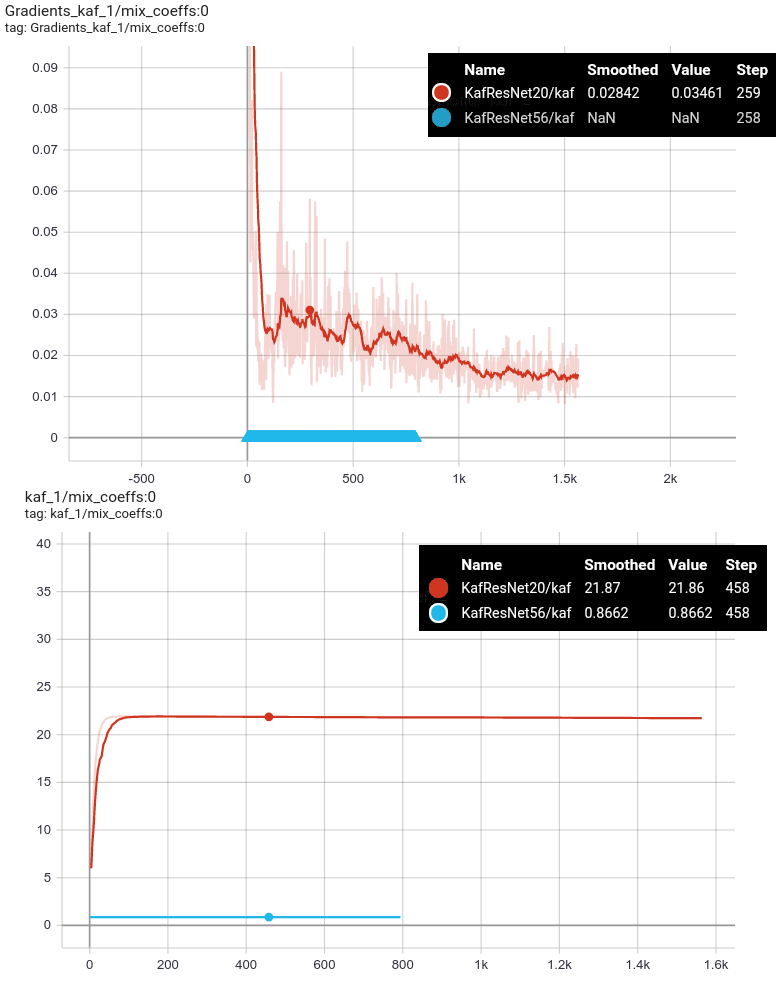
\includegraphics[scale=0.32]{kaf1.png}
            \caption{}
            \label{fig:gradkaf1}
        \end{figure}      
        
        \begin{figure}[h!]
            \centering
            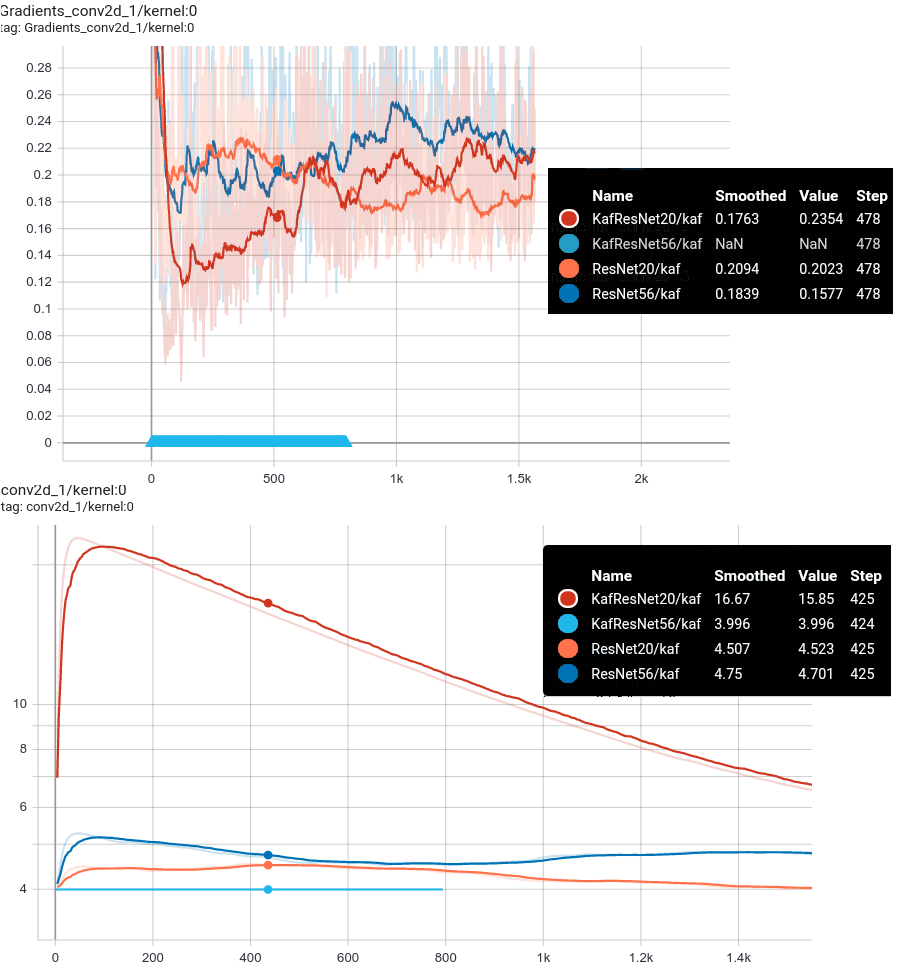
\includegraphics[scale=0.32]{conv1.png}
            \caption{}
            \label{fig:gradconv1}
        \end{figure}
        NaN values are usually the result of unrepresentable operations such as division by zero or the square root of a negative number. In our specific case however, it is more likely that they are generated as a result 
        of vanishing or exploding gradient computation. Indeed, in either case, we would have a weight-update that underflows or overflows the numerical precision in place. Subsequently, the gradient computation for that 
        specific weight will become undefined, producing, from that point backwards, in the backpropagation, only NaN values as the error flows through the network. We are then left to show if the observed NaNs are generating 
        from an exploding or vanishing gradient problem.

        As we continue to analyze deeper layers and their weights, we discover that, around the 15th hidden layer, gradients norm stops being undefined, becoming extremely large instead Fig. \ref{fig:gradkaf15}.
        \begin{figure}[h!]
            \centering
            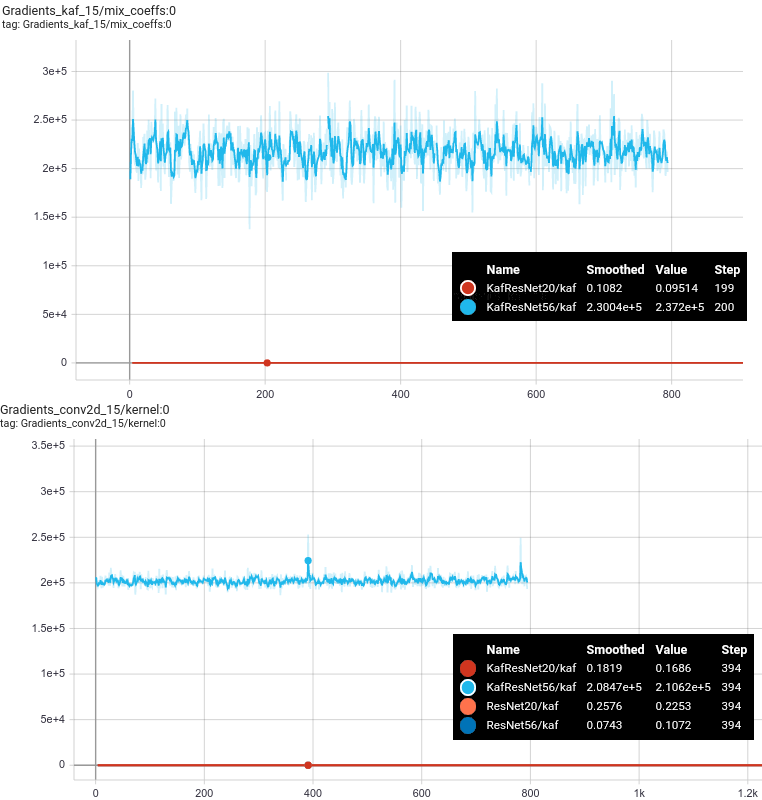
\includegraphics[scale=0.38]{15grad.png}
            \caption{}
            \label{fig:gradkaf15}
        \end{figure} 
        The difference between the plotted norms is strongly noticeable. For both the kernel convolution and the mixing coefficients, KafResnet56 gradients norm is close to $2 \cdot 10^5$, thus being several orders of magnitude 
        bigger than the same norm applied on shallow or ReLU equipped ResNets. The latter norm in fact, fluctuates between 0 and 1, even if it may appear as a straight single-valued line from the plot.

        Our analysis seems to confirm our belief that what is actually happening is a gradient issue, in particular, the extreme grow of gradients which eventually lead to NaN values in the early layers is exaclty the 
        description of exploding gradients, hence the inability to learn.
        
        If we keep plotting towards the last layers, we observe how gradients gradually become more and more close to each-other Fig \ref{fig:gradconv49}.
        \begin{figure}[h!]
            \centering
            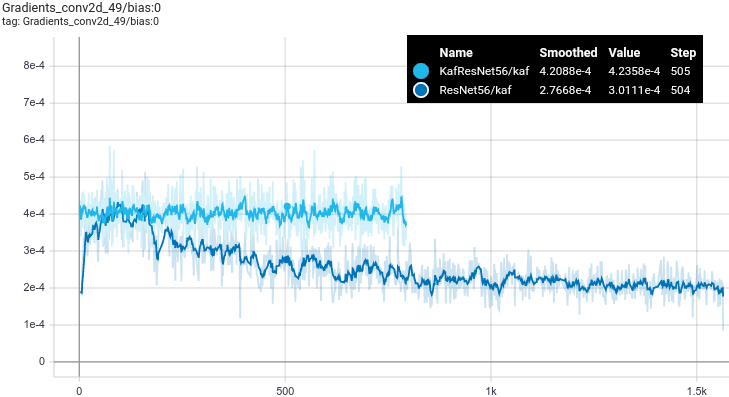
\includegraphics[scale=0.38]{gradconv45.png}
            \caption{}
            \label{fig:gradconv49}
        \end{figure}
        Again, this hints to the fact that exploding gradients is actually caused by the large number of layers employed and not due to some strange, sudden gradient explosion with KAFs.
        More importantly, we deduce that such an issue can be mitigated, if not completely avoided — as for KafResNet20 —, decreasing the number of layers.
        
        Ultimately, it is important to mention that exploding gradients afflict many models in the field of machine learning \cite{gradientproblems_rnn} and thus, as a consequence, many techniques are available nowadays to try to tackle this obstacle. 
        Even if we did try some of them, it is still plausible that a more careful design, such as the use of another kernel method for KAFs specifically targeted to prevent gradient issues, or the adoption of more 
        sophisticated methods such as gradient clipping or spectral-norm regularization \cite{spectralnorm_reg}, might have made possible to train a 56-layered KafNet.  
        The code to reproduce the results discussed in this section can be found in \textit{reskafnets\_n\_exploding\_grads.ipynb}.
    \section{ResNet20 Inspired Architectures Results}

        In order to satisfy the initial requirement on the need for a smooth architecture, that would also be compatible with KAFs, we showed, in the previous section, how a relatively shallow residual neural network is 
        ultimately a good choice. Despite the fact that deeper ResNets achieve better performances \cite{resnet}, using 20 layers is indeed already sufficient to classify correclty the 90\% of the images in our dataset, beating 
        any VGG we previously developed. It is then reasonable to expect better results in terms of accuracy/robustness as well from a ResNet20. Moreover, our main intent is to assess the robustness properties that comes with 
        KAFs and it is not to achieve state-of-the-art results. Therefore, for our last experiment, we decided to evaluate the robustness of a ResNet20, as we change activation functions.

        We follow the same procedure used in the case of VGGs to perform evaluations. Namely, we first adversarially train the network using the enhanced FGSM AT and then a full strength PGD to craft adversarial examples.
        Differently from before, we extended the number of epochs during training to 80 epochs and, importantly, we augment the train set with data augmentation as described in the previous section on exploding gradients.
        The learning rate policy, as well as the optimizer, PGD and KAF hyperparameters are unchanged. The details for the model architecture 
        are again the same provided in the previous section. Finally, the code to reproduce the following results can be found in \textit{fbf\_training\_kafresnets.ipynb}

        In order to give a fair comparison with the VGG case, we evaluate the network with the same set of activation functions, plus 
        a KAF approximation for ReLU (KAF\_ReLU). The outcome of each evaluation is given in Tab. \ref{tab:resnetrob}. Moreover, an accuracy-robustness
        plot Fig. \ref{fig:rob_af2} allows for graphical visualization of each of the produced trade-offs.

        \begin{table*}[!h]
            \centering
            \begin{tabular}{ |p{2.5cm}||p{1.7cm}|p{2.1cm}|  }
                \hline
                \textbf{Activation} & \textbf{Accuracy} & \textbf{Robustness}\\
                \hline
                ReLU & 77.52\% & 50.17\% \\
                ELU & 75.42\% & 51.69\% \\
                KAF & 78.08\% & 52.23\% \\
                KAF\_ReLU & \textbf{79.65}\% & 51.44\% \\
                KAF\_ELU & 78.69\% & 52.76\% \\
                Swish & \underline{78.68\%} & \underline{\textbf{53.88\%}} \\
                KAF\_Swish & 79.21\%& 52.10\% \\
                KAF\_Free & 78.88\%& 52.07\% \\
                \hline
            \end{tabular}
            \caption{Summary of the robustness gained from changing activation functions in an 
            adversarially trained ResNet20. Bold denotes best result while underline best trade-off.}
            \label{tab:resnetrob}
        \end{table*}
        \begin{figure}[!h]
            \centering
            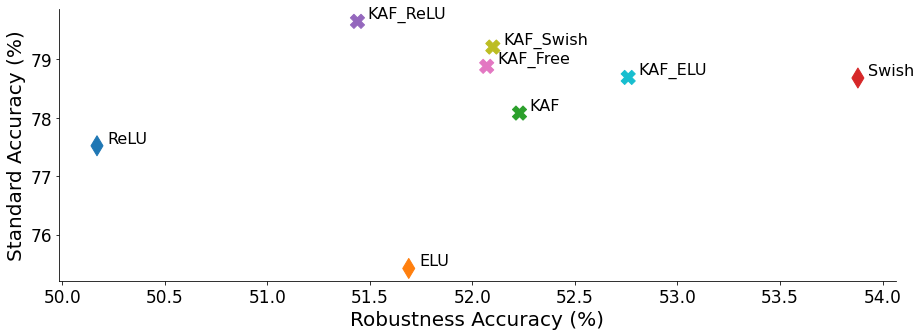
\includegraphics[width=0.8\textwidth]{rob_af2.png}
            \caption{Robustness/accuracy visualization for a ResNet20 equipped with different activation functions. 
            Fixed activation functions are shown with a thin diamond whereas non-parametric KAFs with a filled x. Swish achieves best robustness and KAFs generally tend 
            to improve both robustness and accuracy with respect to a ReLU baseline.}
            \label{fig:rob_af2}
        \end{figure}


        Before we start to comment on each single activation function's score, it is important to remark how, regardless of the 
        activation function being used, the network significantly improves in robustness over the VGG case. In fact, even in the least 
        performant case -- corresponding to the ReLU baseline --, we are still outperforming the best 47.73\% robustness obtained
        with Swish equipped VGG. This highlights the importance of choosing the right architecture, which in our case corresponded to 
        a non-smooth component-free architecture, adding value to the smoothness thesis. Moreover, note how this comparison is especially
        meaningful since the standard accuracies and the total number of weights between the two architectures are nearly the same, therefore,
        given equal resources, the ResNet seems to be really more robust.

        A second key point to highlight concerns how, this time, ReLU is definitely acting as a base line.
        Indeed, any of the tested smooth activation functions, even the ELU, manages to substantially 
        increase the robustness of the network with respect to the 50.17\% achieved by ReLU. Again, 
        this behavior is in line with \cite{smooth_adversarial_training} evaluations. 
        
        Furthermore, extending \cite{smooth_adversarial_training}
        observations, we discover that, in a much noticeable way than with VGG, the usage of KAFs 
        in ResNet20 always results in a boost in standard accuracy, wether we consider the baseline 
        but, more in general, it applies to any fixed activation function since, approximating the  
        initial shape of a KAF with a fixed activation function leads, in every instance, to greater 
        accuracies Fig. \ref{fig:rob_af2}.

        Ultimately, the most remarkable result for our study concerns the robustness obtained 
        with Swish functions. Achieving a total robustness of 53.88\% and thus improving 
        by a margin of almost 4 points from the baseline and also considerably from the second-bestperforming functions (KAF\_ELU), Swish is confirmed once again as the 
        preferable function to pick for maximizing the robustness of a deep neural network. 
        Moreover, Swish performs reasonably well in terms of standard accuracy too, being less than one point away 
        from the maximum reached with KAF\_ReLU. Therefore, after having evaluated several activation 
        functions and structurally different architectures, we argue that is typically convenient to 
        choose Swish activation functions when we want to build a robust neural network.



\chapter{Conclusions and Future Works}

        \label{chap:8}
        \section{Conclusions}

        In this thesis, we addressed the problem of the importance of activation functions for the robustness of deep neural networks, 
        with particular emphasis on the class of non-parametric activation functions known as kernel-based activation functions (KAFs).
        Our initial hypothesis on the potential of KAFs in improving adversarial robustness was only marginally validated by the experiments we made. Even though
        it is still plausible that a fine-grained optimization of hyperparameters such as the dictionary size or the kernel-bandwidth,
        or even the regularization of the mixing coefficients, might have led to stronger results, we conclude that the main reason behind the 
        observed lack in effectiveness, is to be found in the properties of the KAF itself. That is, as much as a user can exploit 
        smoothness and flexibility to improve accuracy and, in particular, to strength adversarial training, we should not forget that this also holds 
        true from the adversary side. Enhanced flexibility means more resiliency against attacks, but it also means more space for the attacker to 
        search for even stronger adversarial examples. The addiction of non-linearity in the output space of $f_{\theta}$ that comes with KAFs, can in fact
        be leveraged by any gradient-based attack, including PGD. On the contrary, fixed activation functions do not introduce new parameters or flexibility in the network. Therefore,
        only through smoothness, we can train a model against strong attacks, that cannot, loosely speaking, be made stronger by any adversary.
        It is this lack of unbalanceness towards the defense side that is missing with KAFs, preventing them to overcome, for instance, the performance of Swish activation functions.

        As a side effect, the results reported in this thesis can also serve as a contribution to the bag of evidence for 
        some of the related works that we mentioned and used, especially for those recent ones, which may benefit from additional 
        empirical validations. Specifically, from the VGG and ResNet robustness evaluations, it clearly emerged how KAFs are likely to improve
        the generalization properties over fixed activation functions, as first described in \cite{kafnets}.
        Similarly, in these experiments we also find that the Swish activation function consistently outperforms 
        other activation functions in terms of robustness, giving credits to \cite{smooth_adversarial_training}. Lastly, we were able to implement
        the fast adversarial training method described in \cite{fast_adv_train} in another framework and still matching the reported
        running-times.

        \section{Future Works}

        Many different ideas, extensions, and experiments have been left for the future due to the lack of time and resources. In particular, the following is a list of tracks that deserve to be tested:
        \begin{itemize}
            \item Despite KAFs did not stand out as the optimal activation function to be used in an adversarial training scenario, it is worth recalling that adversarial training is just one 
            out of different known methods to tackle the problem of Robust Optimization. Another approach that is known to be effective and in which KAFs might find a successful
            application, is the area of certified defenses. In such particular setting, the flexibility of KAFs might be exploited to devise defenses that are provable to be secure against 
            norm-bounded perturbations. In this regard, authors in \cite{lipschitz_train} propose a training procedure to enlarge the provably guarded area around data points 
            by means of a minimization of the Lipschitz constant of the network. In \cite{coello2003micai} an explicit upper bound for the Lipschitz
            constant of a KAF is given.

            \item Previously known to be a computationally prohibitive task to accomplish, the adversarial training of a deep neural network for ImageNet is now becoming ever more accessible 
                  due to the progress of the hardware and the development of efficient procedures such as the FSGM adversarial training used \cite{fast_adv_train}. Therefore, scaling the experiments discussed in this thesis
                  to ImageNet to check if the results are coherent with those of CIFAR10 is advisable. 

            \item Other than PGD, perform other famous attacks such as C\&W, DeepFool or, more importantly, \textit{adaptive attacks} to assess the robustness of adversarially trained Kafnets. 
            Adaptive attacks are attacks that were specifically designed to target a given defense and it has nowadays become the standard to perform true robustness evaluations \cite{towards_eval_robustness}.
            Indeed, just as was shown for k-WTA \cite{carlinikwta}, there may be a subtle gradient-based attack which could target the presence of trainable activation functions in the network 
            to produce adversarial examples capable of making adversarial training worse than when using, for instance, ReLU activation functions. Several best practices have been proposed to help spot possible flaws 
            in a defense and design adapative attacks \cite{carlinikwta}.
        \end{itemize}
            

    
   
    
\appendix


\backmatter
% bibliography
%\cleardoublepage
%\phantomsection
%\bibliographystyle{sapthesis} % BibTeX style
%\bibliography{bibliography} % BibTeX database without .bib extension
\printbibliography

\end{document}
